% !TeX root = syllabus_ELEC0053.tex
% !TeX encoding = ISO-8859-1
% !TeX spellcheck = fr_FR

\section{Exercices}


\begin{exercise}{}
	\label{ex:2-3}
On considère le circuit suivant 
\begin{center}
	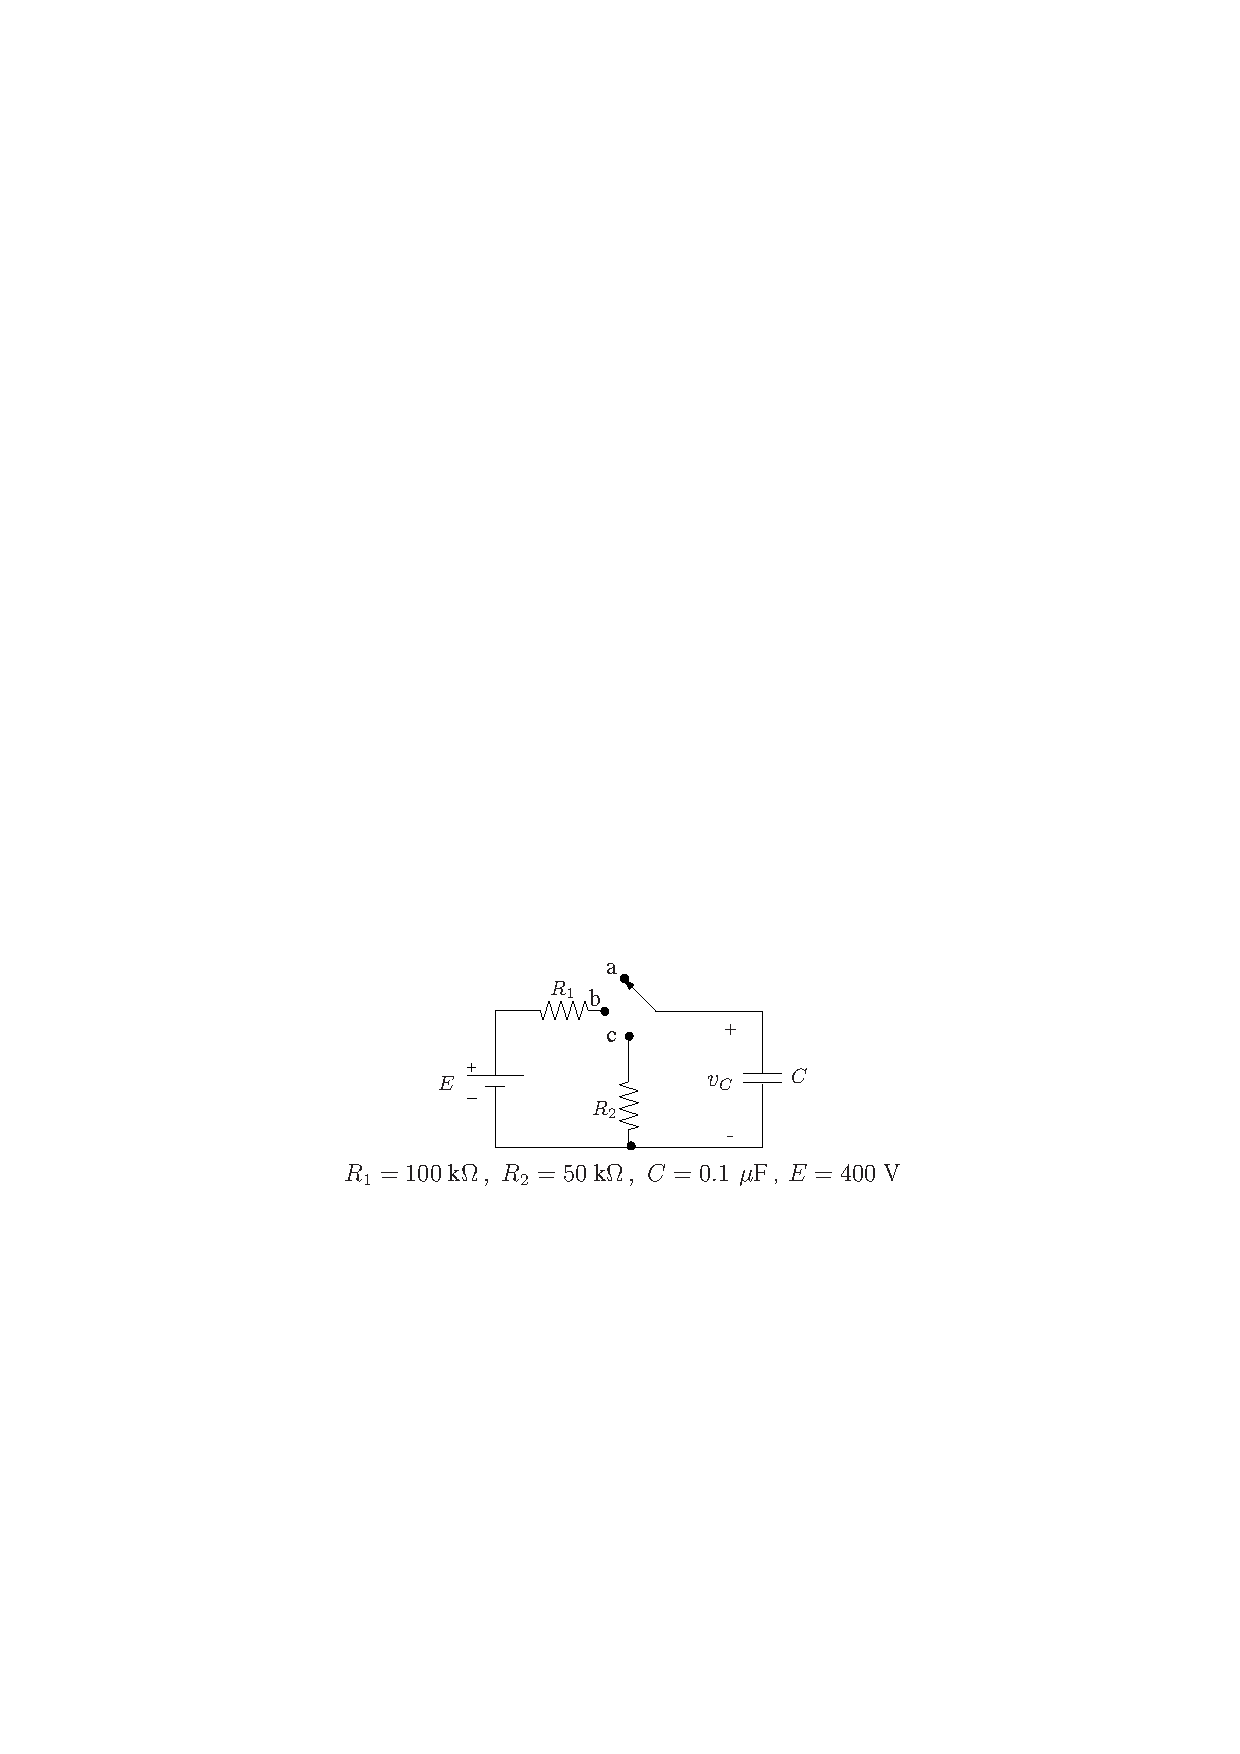
\includegraphics[width=0.85\linewidth]{exercices/ex-3-3}
\end{center}
et les conditions de fonctionnement suivantes :
\begin{enumerate}
	\item l'interrupteur est initialement en position a, le condensateur
	étant initialement relaxé;
	\item à l'instant  $t=0$, l'interrupteur bascule en position b et y reste pendant 15 ms;
	\item à l'instant  $t=15$ ms, l'interrupteur bascule en position c et y reste indéfiniment. 
\end{enumerate}
Dans ces conditions :
\begin{enumerate}
	\item dériver l'expression numérique de la tension $v_C$ aux bornes du condensateur;
	\item tracer le graphe de $v_C(t)$;
	\item déterminer le ou les instant(s) auxquels la tension $v_C(t)$ est égale à 200 V.
\end{enumerate}
\rep{1. $v_C(t)=400(1-e^{-100t})$ V, $0\leq t < 15$ ms \\ $v_C(t)=310.75e^{-200(t-0.015)}$ V, $t \geq 15$ ms \\
3. $t_1=6.93$ ms, $t_2=17.2$ ms}
\end{exercise}

\begin{exercise}{}
	\label{ex:2-5}
Déterminer la réponse libre du circuit suivant
\begin{center}
	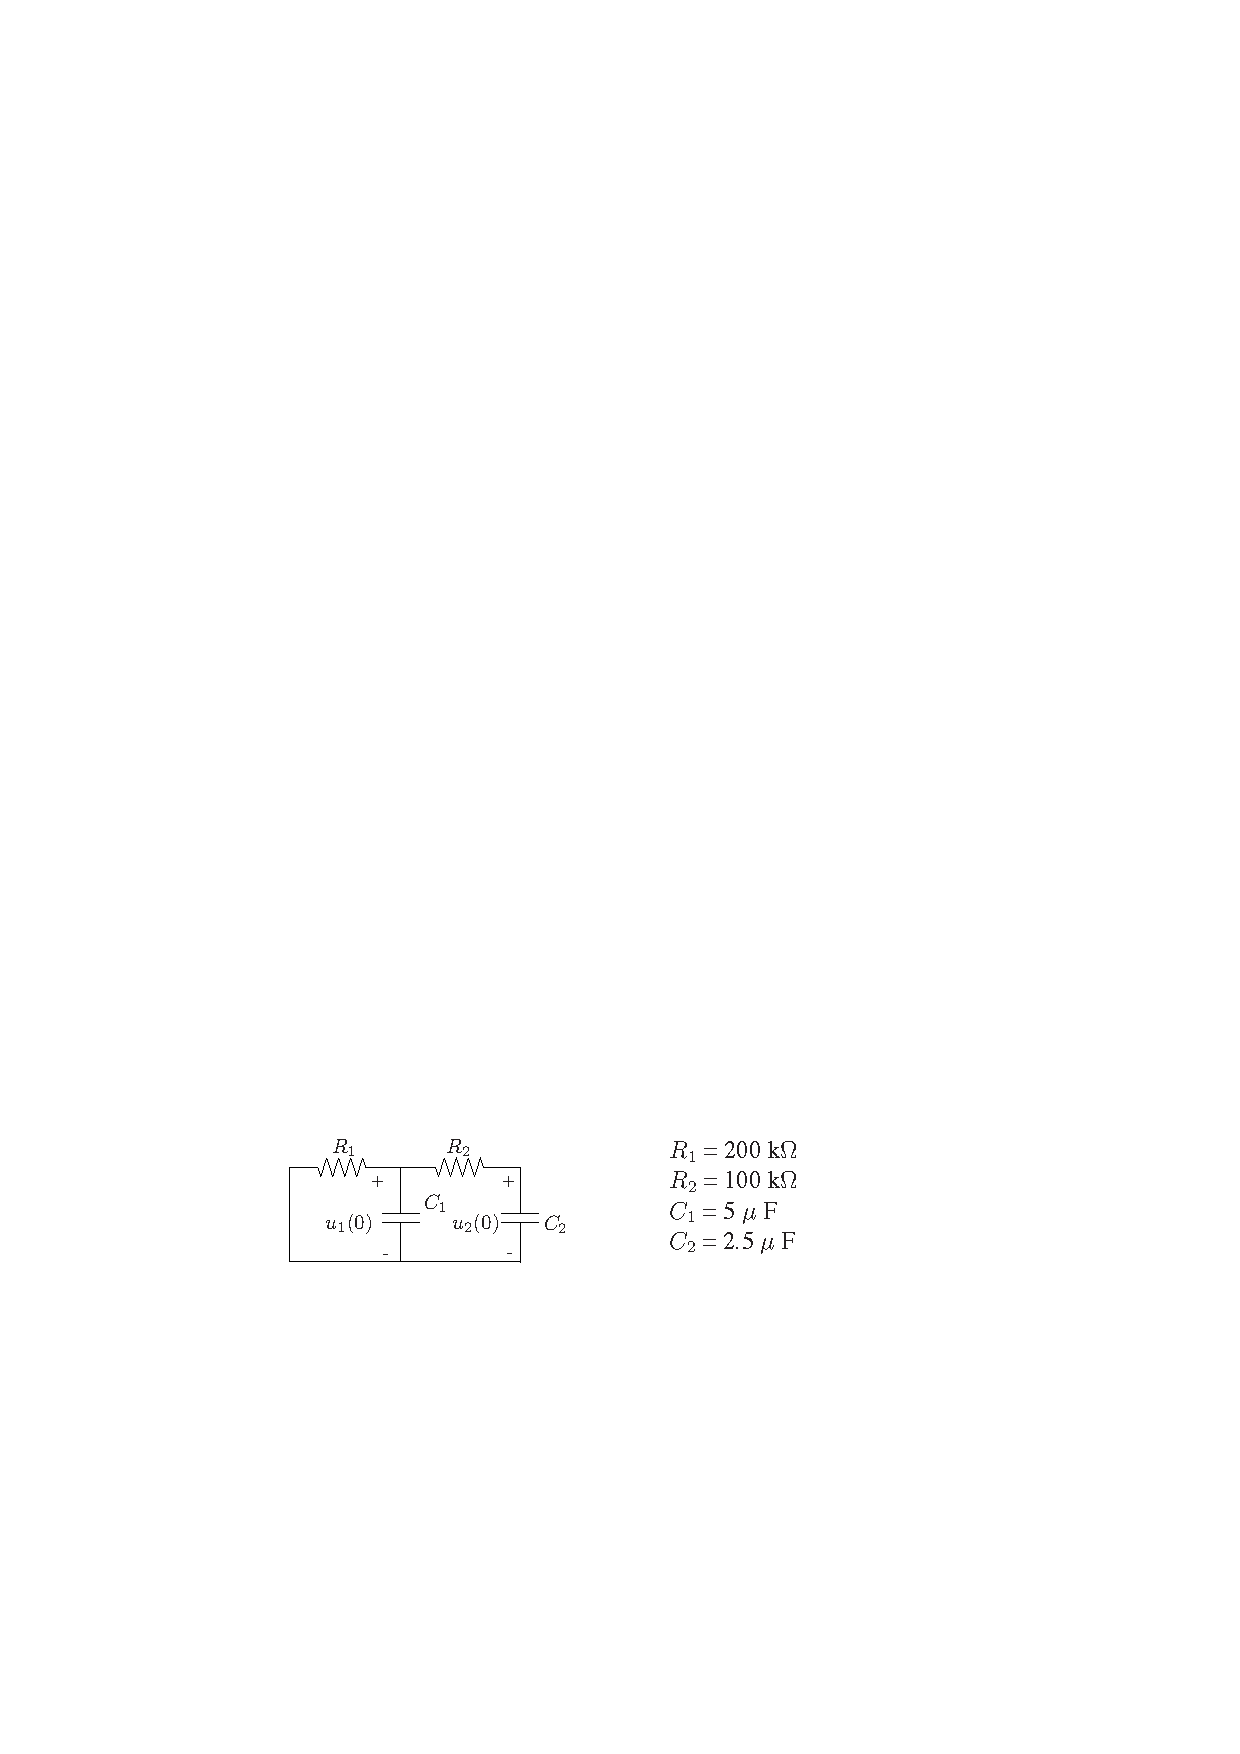
\includegraphics[width=0.8\linewidth]{exercices/ex-3-5}
\end{center}
en fonction des conditions initiales :
\begin{eqnarray*}
	u_1(0)&=&2V\\
	u_2(0)&=&5V\\
\end{eqnarray*}


\rep{$u_1(t)=2.9e^{-0.63 t}-0.91e^{-6.37 t}$ V \\
$u_2(t)=3.46e^{-0.63 t}+1.54e^{-6.37 t}$ V}
\end{exercise}

\begin{exercise}{}
	\label{ex:2-6}
On considère le circuit ci-dessous.
\begin{center}
	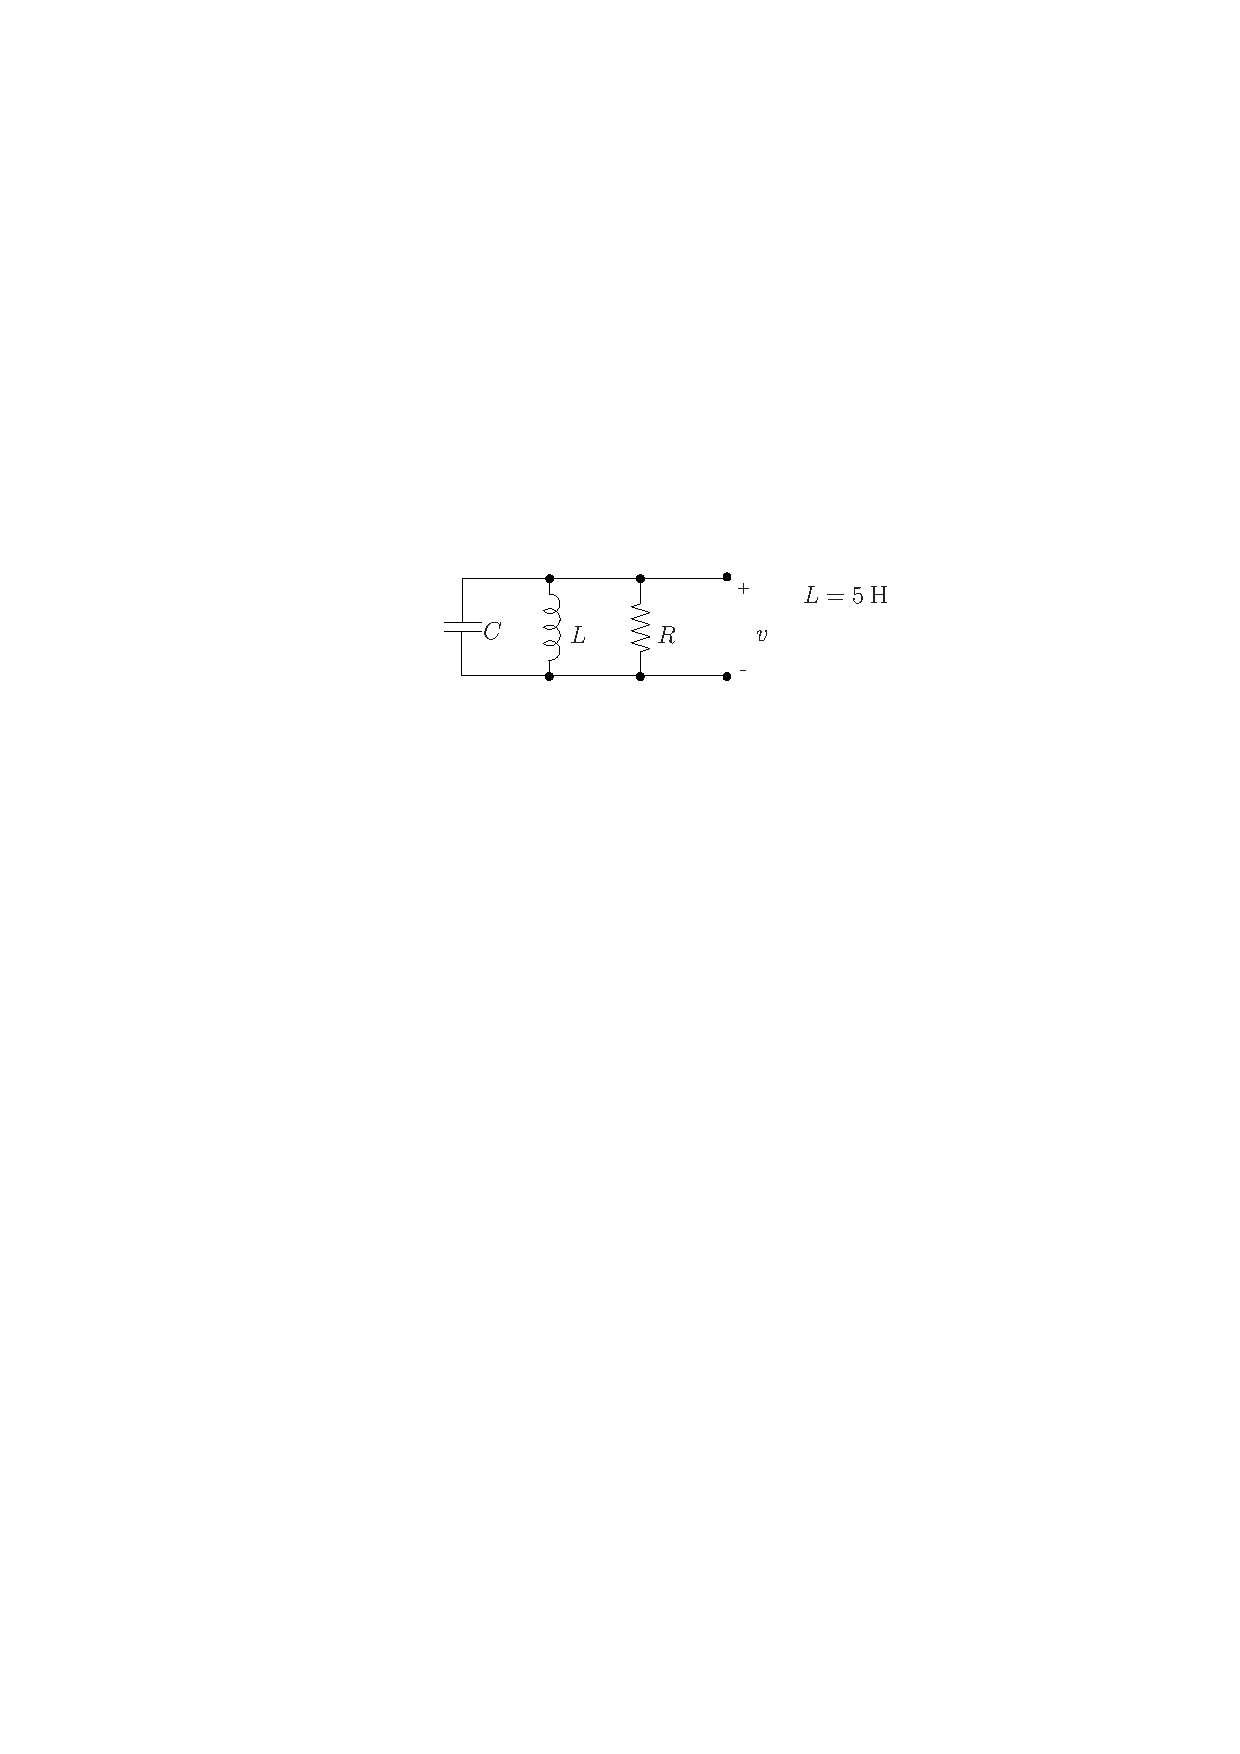
\includegraphics[width=0.6\linewidth]{exercices/ex-3-6}
\end{center} 
Si la tension aux bornes de ce circuit s'écrit :
\[v(t)=D_1te^{-4000t}+D_2e^{-4000t}\,\, \mbox{V}, t\geq 0\]
déterminer la valeur des deux éléments $R$ et $C$ ainsi que des deux
coefficients $D_1$ et $D_2$ sachant que :
\begin{enumerate}
	\item le courant initial $i_0$ parcourant l'inductance est égal à 5 mA;
	\item la tension initiale $v_0$ aux bornes du condensateur est égale à 25 V.
\end{enumerate}
\rep{$R=10$ k$\Omega$ , $C=12.5$ nF , $D_1=-5\, 10^5$ , $D_2=25$.}
\end{exercise}


\begin{exercise}{}
	\label{ex:2-7}
On considère le circuit ci-dessous. 
\begin{center}
	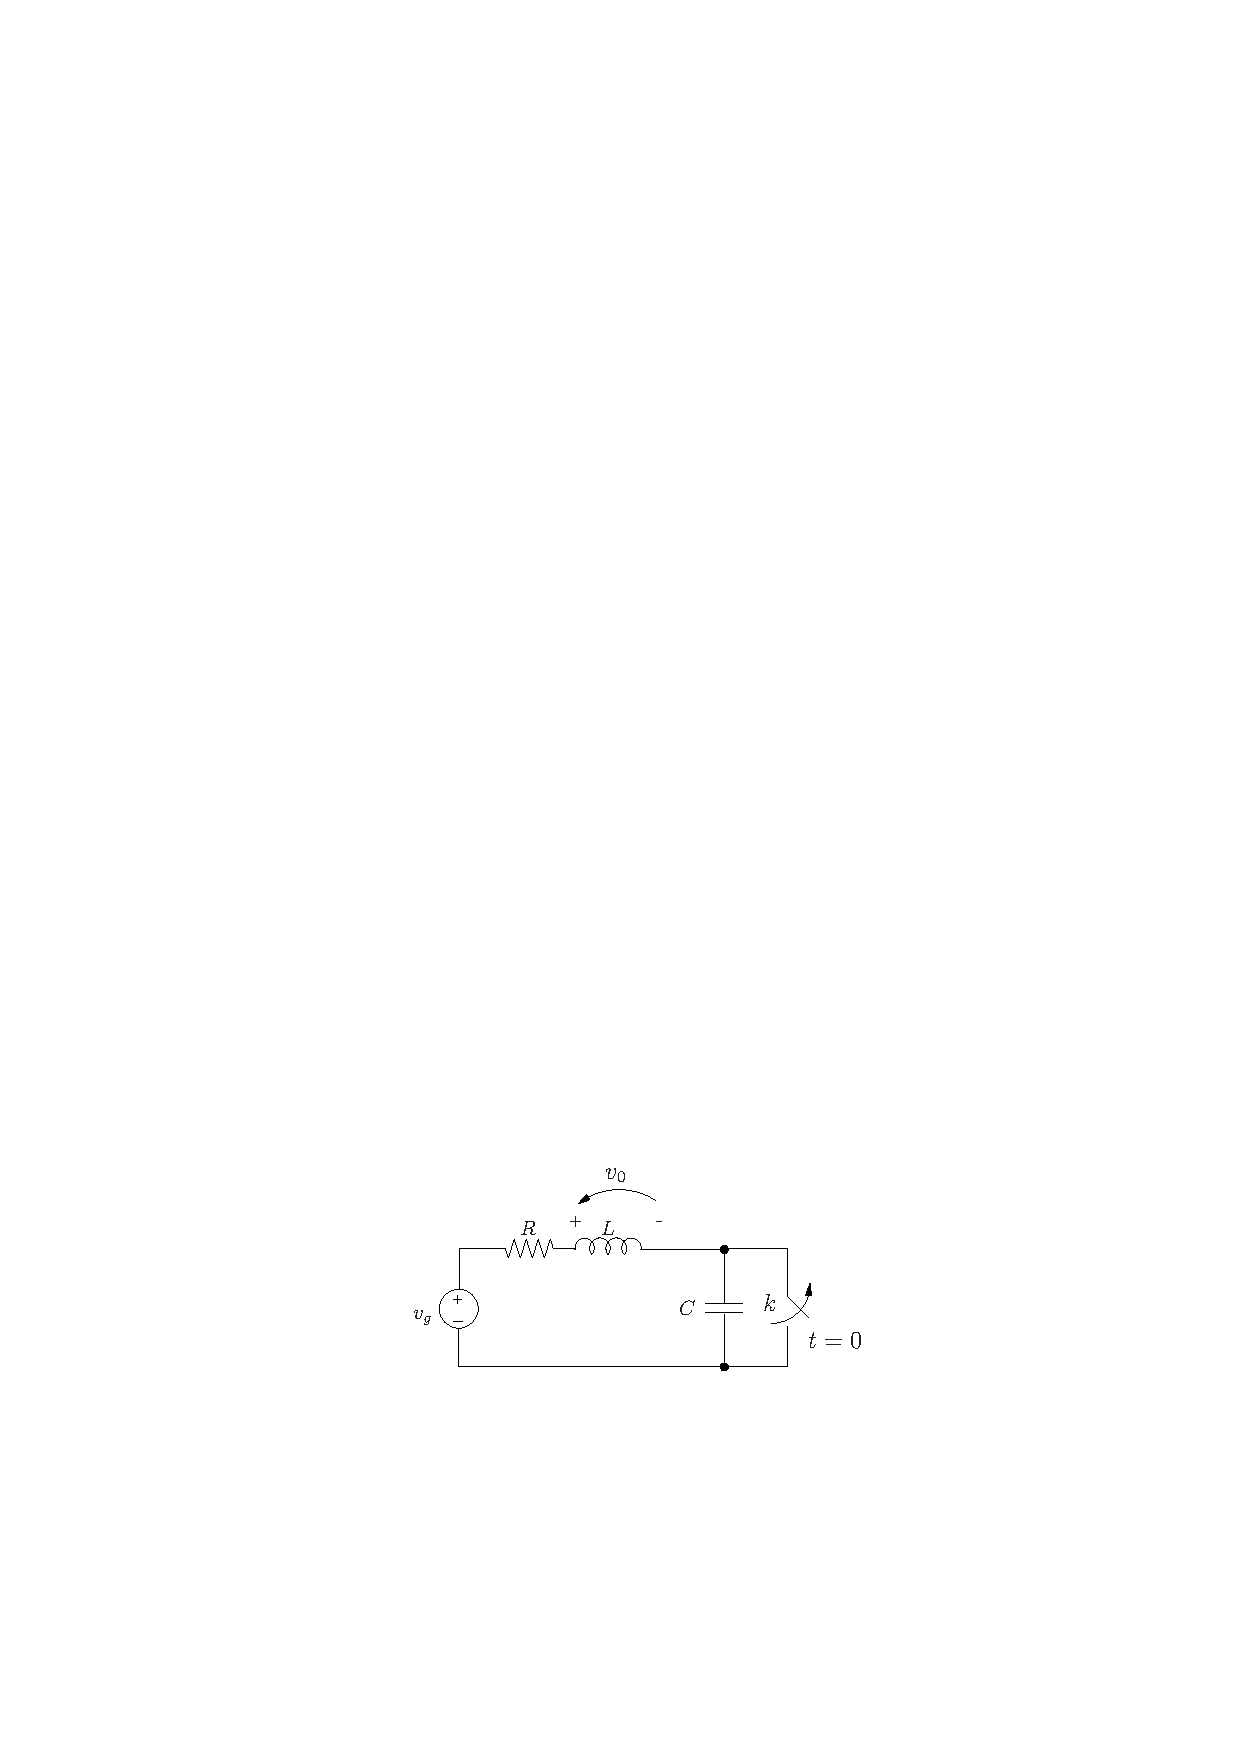
\includegraphics[width=0.5\linewidth]{exercices/ex-3-7}
\end{center}
L'interrupteur
$k$ est supposé fermé depuis un temps infini. A l'instant $t=0$ il
s'ouvre. On suppose que les valeurs des éléments du circuit sont telles
que la réponse est de type oscillatoire amorti.  Dériver l'expression
de $v_0(t)$ pour $t\geq 0$ en fonction des paramètres $v_g$, $\alpha$ et 
$\omega_d$.

\rep{$v_0(t)=-v_g(\frac{\omega_d}{2\alpha}+\frac{\alpha}{2\omega_d}) e^{-\alpha t}\sin \omega_d t$ V, $t\geq 0$.}
\end{exercise}

\begin{exercise}{}
	\label{ex:2-8}
\begin{center}
	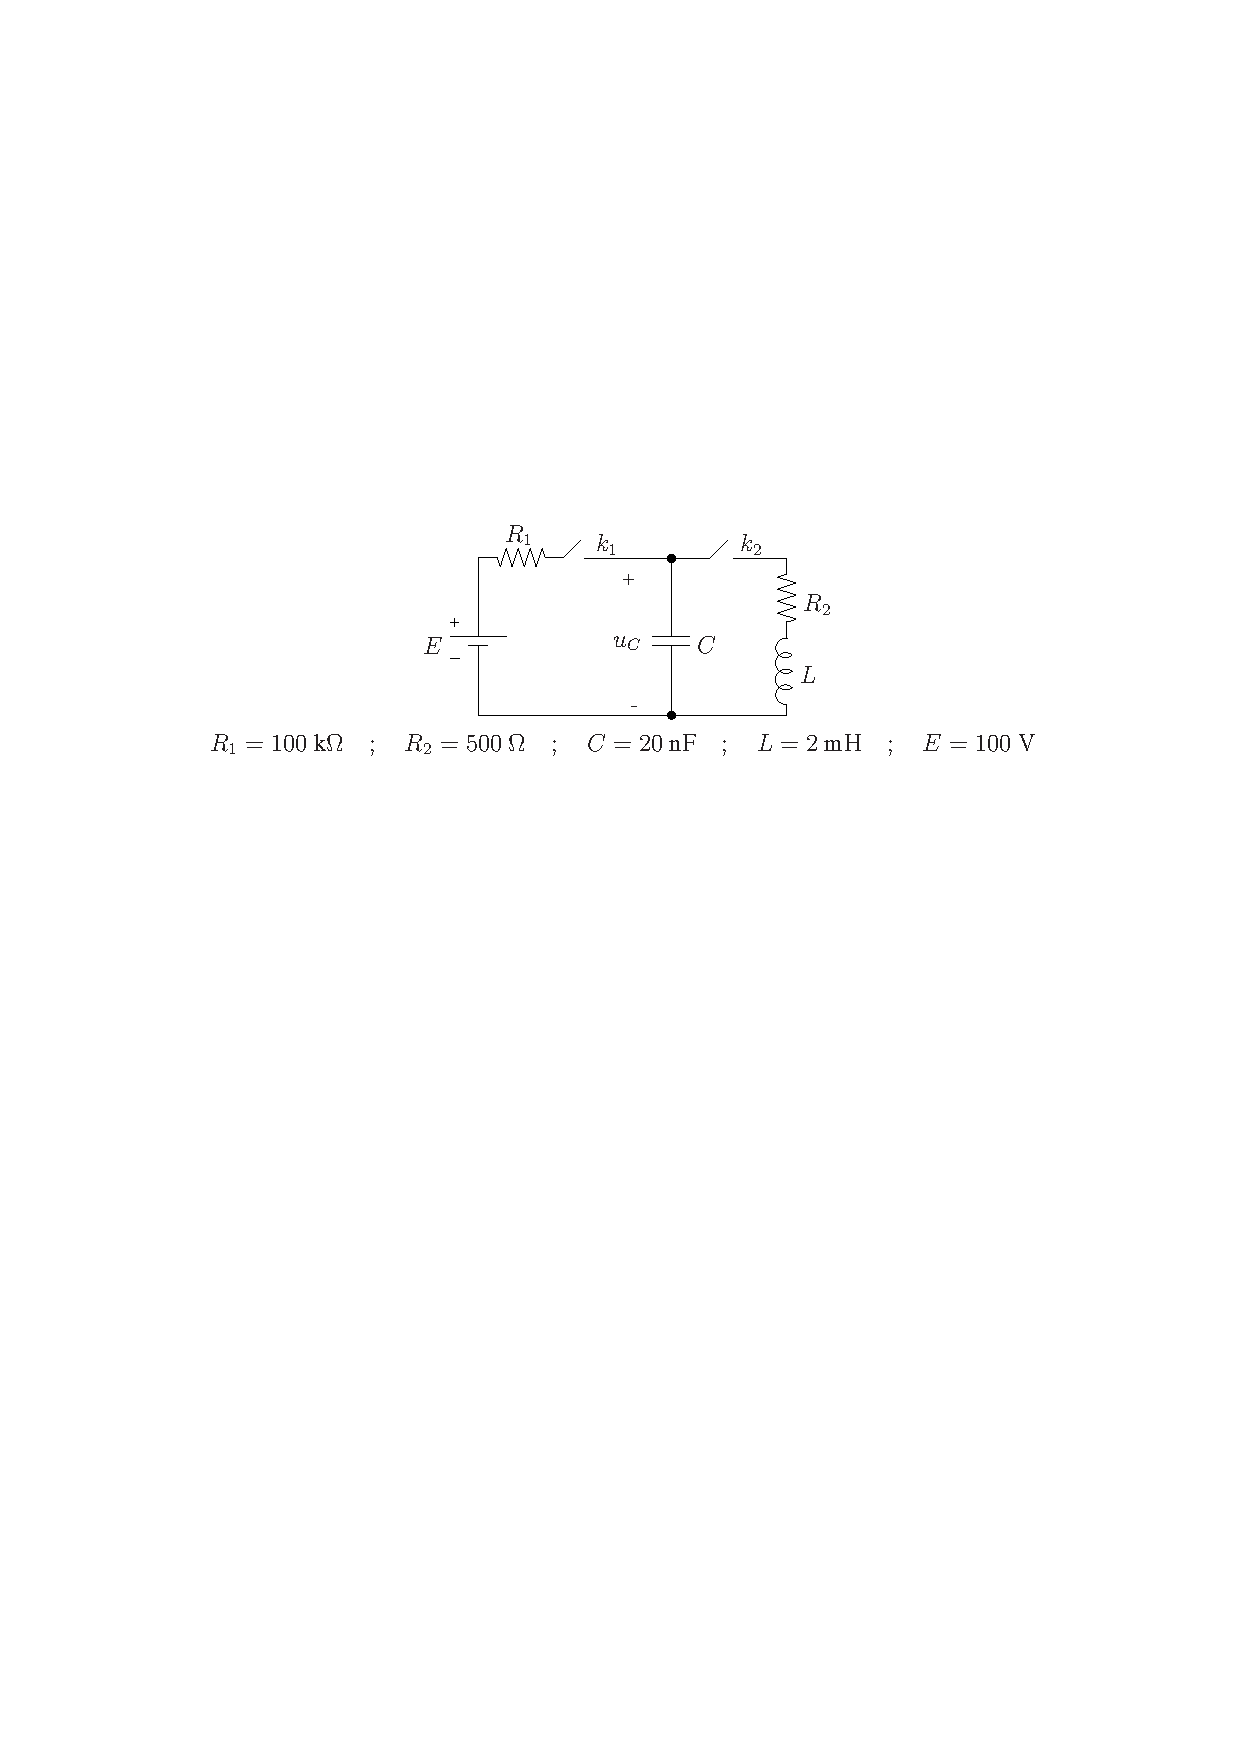
\includegraphics[width=0.95\linewidth]{exercices/ex-3-8}
\end{center}
Le circuit ci-dessus est initialement relaxé, les deux
interrupteurs $k_1$ et $k_2$ ouverts. 
\begin{enumerate}
	\item A l'instant $t=0$, l'interrupteur $k_1$ se ferme, $k_2$ reste
	ouvert.
	\item A l'instant où la tension $u_C(t)$ aux bornes du condensateur
	atteint 90\% de la valeur finale qu'elle atteindrait si on laissait
	le régime s'établir, l'interrupteur $k_1$ s'ouvre et $k_2$ se ferme.
\end{enumerate}
On demande de déterminer l'évolution de la tension $u_C(t)$ pour $t>0$.

\rep{$u_C(t)= 100(1-e^{-500t})$ V, $0\leq t < 4.6\,10^{-3}$ s \\
$u_C(t)= 147 e^{-1.25\,10^5(t-4.6\, 10^{-3})}\sin (9.68\, 10^4(t-4.6\, 10^{-3})+0.66)$
V, $t \geq  4.6\,10^{-3}$.}
\end{exercise}


\begin{exercise}{} \label{ex:2-9}
On désire procéder au lancement d'un moteur à courant
continu en insérant une résistance de démarrage $R_d$. Cette
résistance est mise hors-circuit lorsque le courant délivré par la
source devient inférieur à 15 A. On supposera un temps mort de 0.05 s
pour la mise hors circuit de la résistance. Le moteur est modélisé par
un schéma équivalent simplifié constitué d'une force
contre-électromotrice, d'une résistance et d'une  inductance comme
indiqué dans la figure suivante.
\begin{center}
	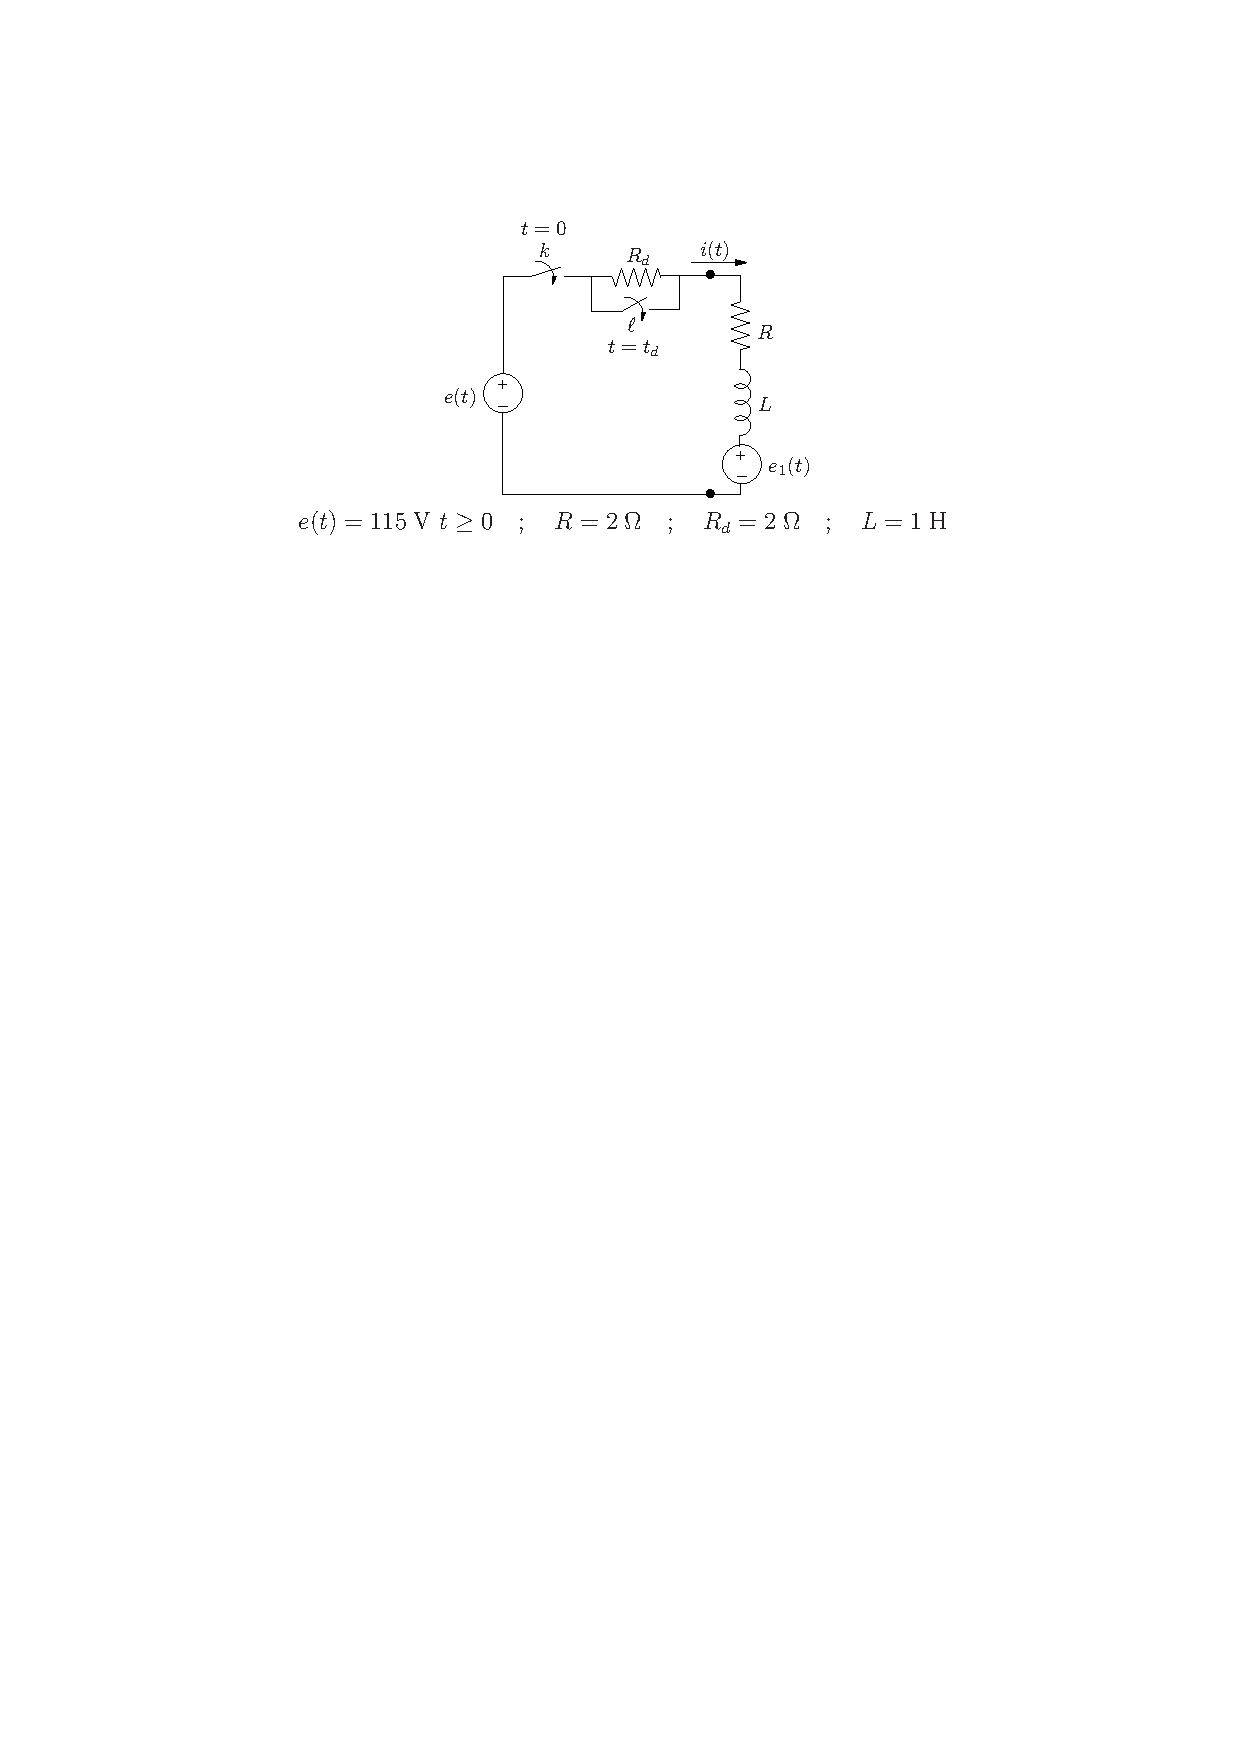
\includegraphics[width=0.9\linewidth]{exercices/ex-3-9}
\end{center}
La force contre-électromotrice est supposée avoir la forme suivante :
\[e_1(t)=100(1-e^{-t/1.5})\,\, \mbox{V}\]

Déterminer l'évolution du courant $i(t)$ pour $t>0$.

\rep{
$i(t)=3.75 - 33.75 e^{-4t}+30e^{-\frac{2}{3}t}$ A, $0 \leq t < 1.51$ s \\
$i(t)=7.5 - 414.2 e^{-2t}+75e^{-\frac{2}{3}t}$ A, $t \geq 1.51$ s}
\end{exercise}

\begin{exercise}{}
	\label{ex:2-11}
	\begin{center}
		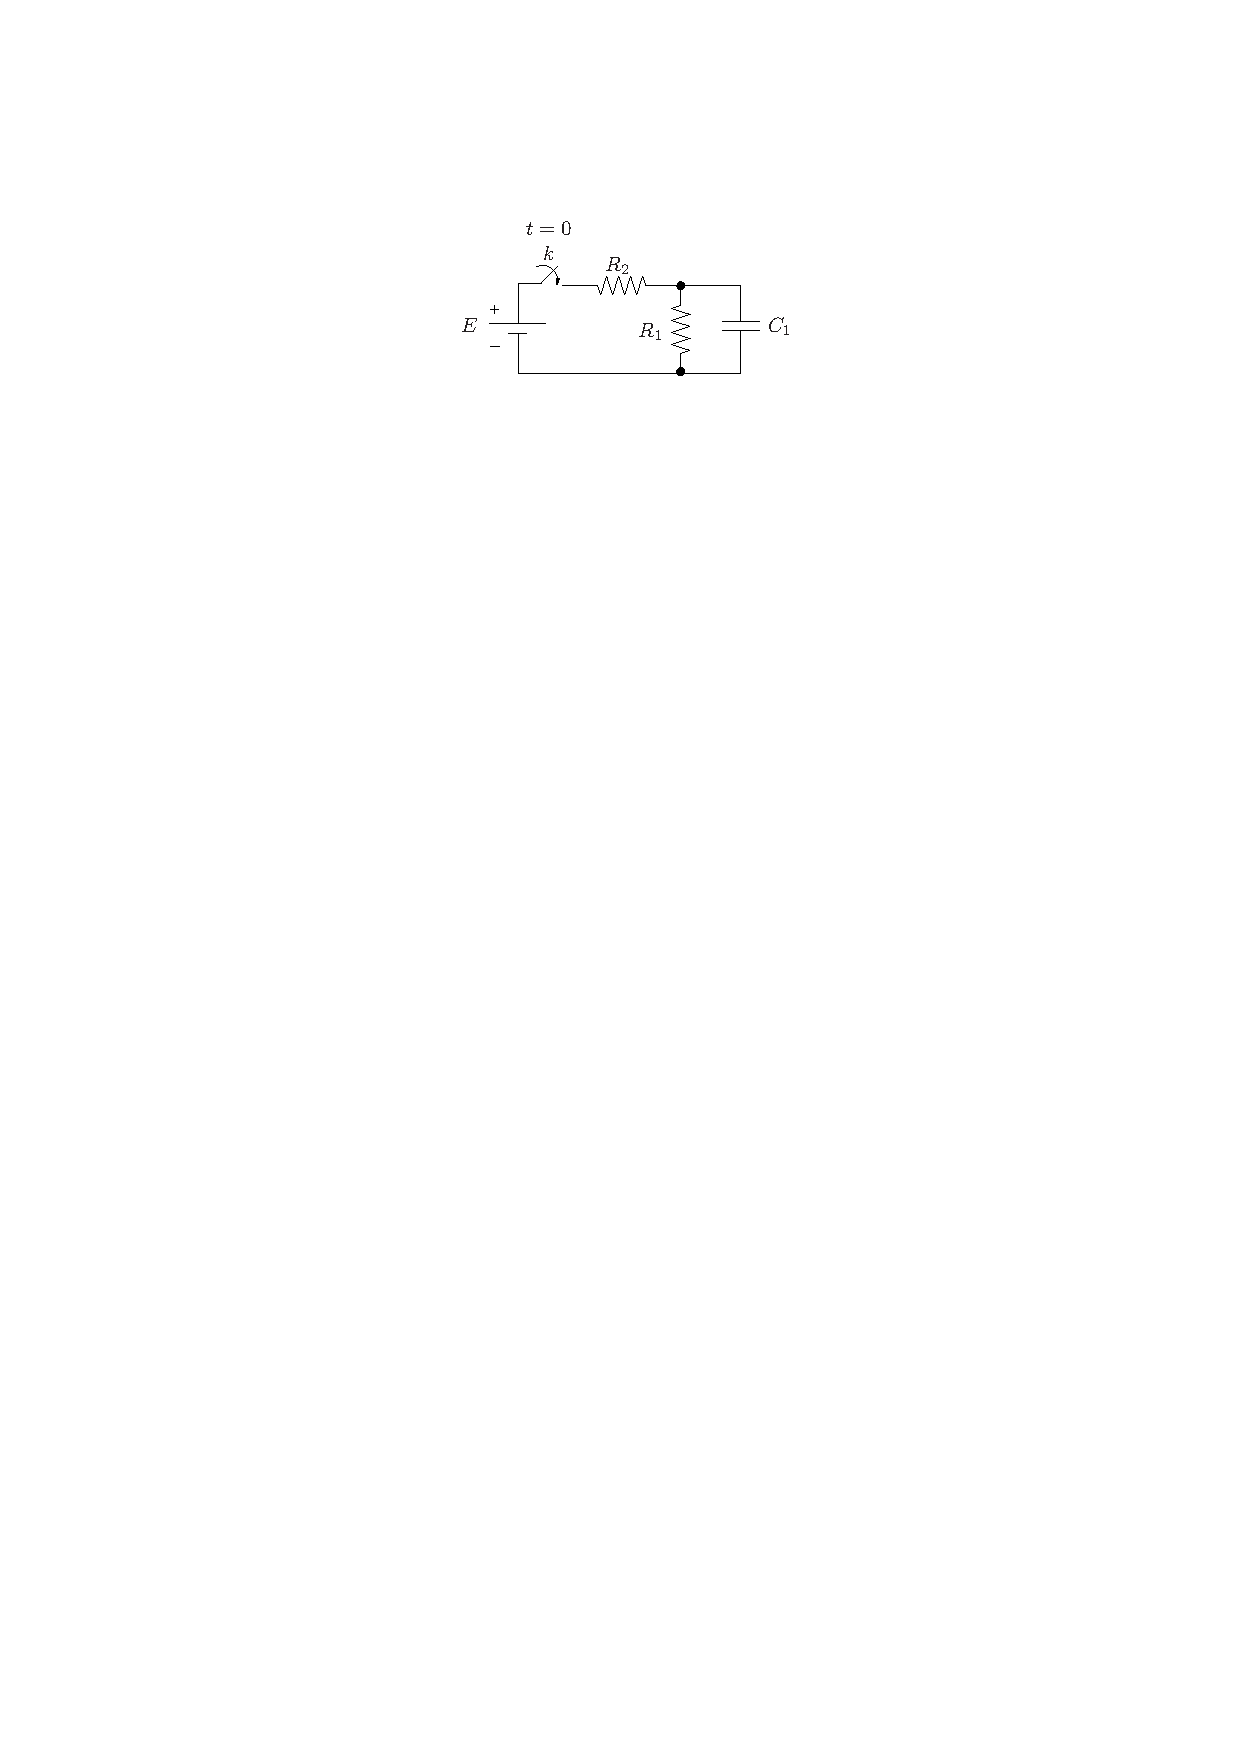
\includegraphics[width=0.6\linewidth]{exercices/ex-3-11}
	\end{center}
	On considère le circuit de la figure ci-dessus et on demande de
	déterminer l'évolution de la tension $v_{C_1}(t)$ aux bornes du
	condensateur $C_1$ si :
	\begin{itemize}
		\item le condensateur est initialement porté au potentiel $v_0$
		\item l'interrupteur $k$ est fermé en $t=0$.
	\end{itemize}
	
	\rep{$v_{C_1}(t)= E\,\frac{ R_1}{ R_1+R_2}(1-e^{-t/\tau})+v_0 e^{-t/\tau}$ V, 
		$t\geq 0$}
\end{exercise}

\begin{exercise}{}
	\label{ex:2-14}
	\begin{center}
		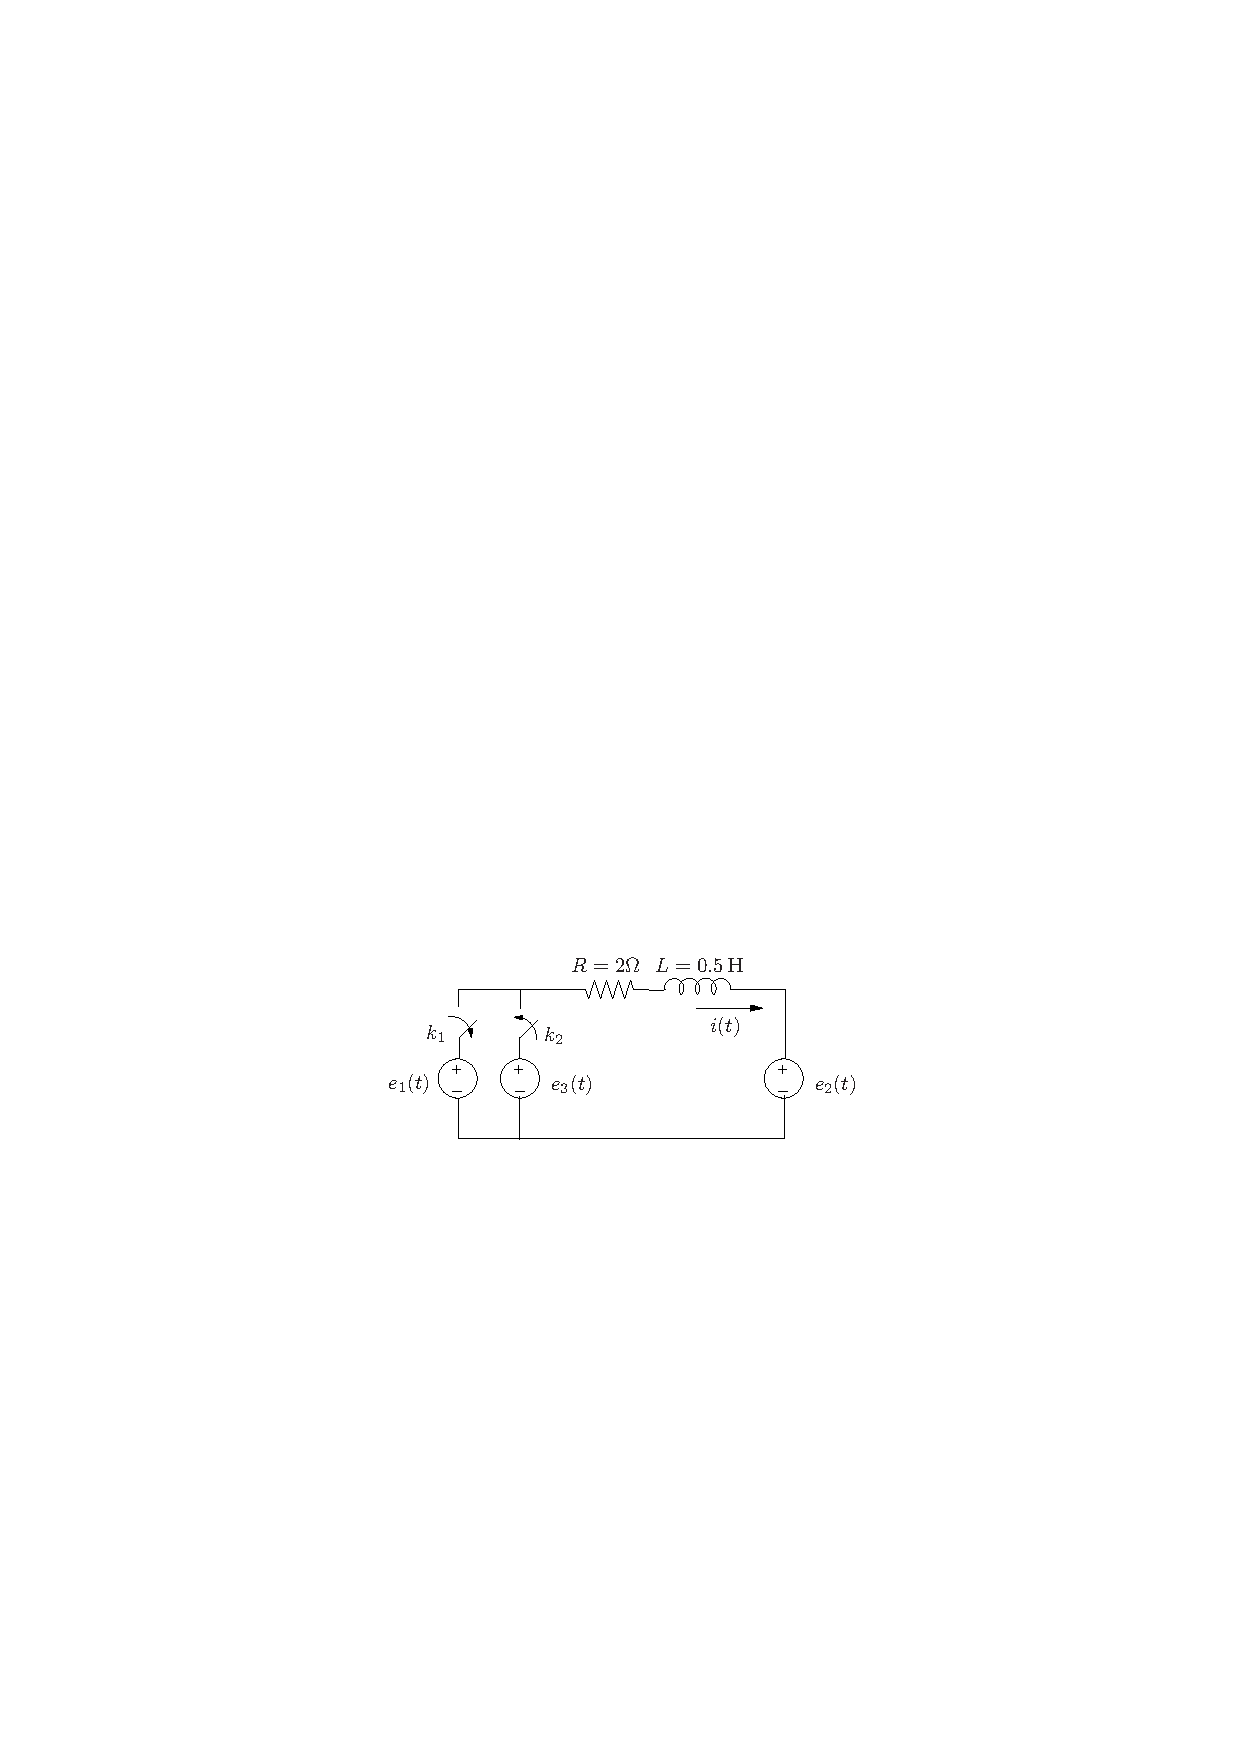
\includegraphics[width=0.6\linewidth]{exercices/ex-3-14}
	\end{center}
	
	On considère le circuit ci-dessus et les conditions de
	fontionnement suivantes :
	\begin{enumerate}
		\item depuis un temps supposé infini, le régime est établi avec
		l'interrupteur $k_1$ fermé et l'interrupteur $k_2$ ouvert
		\[e_1=120\mbox{~V}\quad;\quad e_2=100\mbox{~V}\]
		\item à l'instant $t=0$, la f.e.m. $e_1$ commence à décroître selon
		\[e_1(t)=120e^{-10t}\]
		\item soit $t_0$ l'instant où le courant $i(t)$ s'annule;
		\item après un temps mort de 0.05s, soit à l'instant $t_d=t_0+0.05$,
		l'interrupteur $k_1$ s'ouvre et l'interrupteur $k_2$ se ferme, et
		\[e_3=120 \mbox{~V}\]
	\end{enumerate}
	Déterminer dans ces conditions l'évolution du courant $i(t)$.
	
	\rep{$i(t)=100e^{-4t}-50 -40e^{-10t}$ A, $0\leq t < 0.17$ s\\
		$i(t)=10-32.48e^{-4t}$ A, $ t \geq 0.17$ s}
\end{exercise}

\section{Exercices non résolus}

\begin{exercise}{}
	\label{ex:2-12}
\begin{center}
	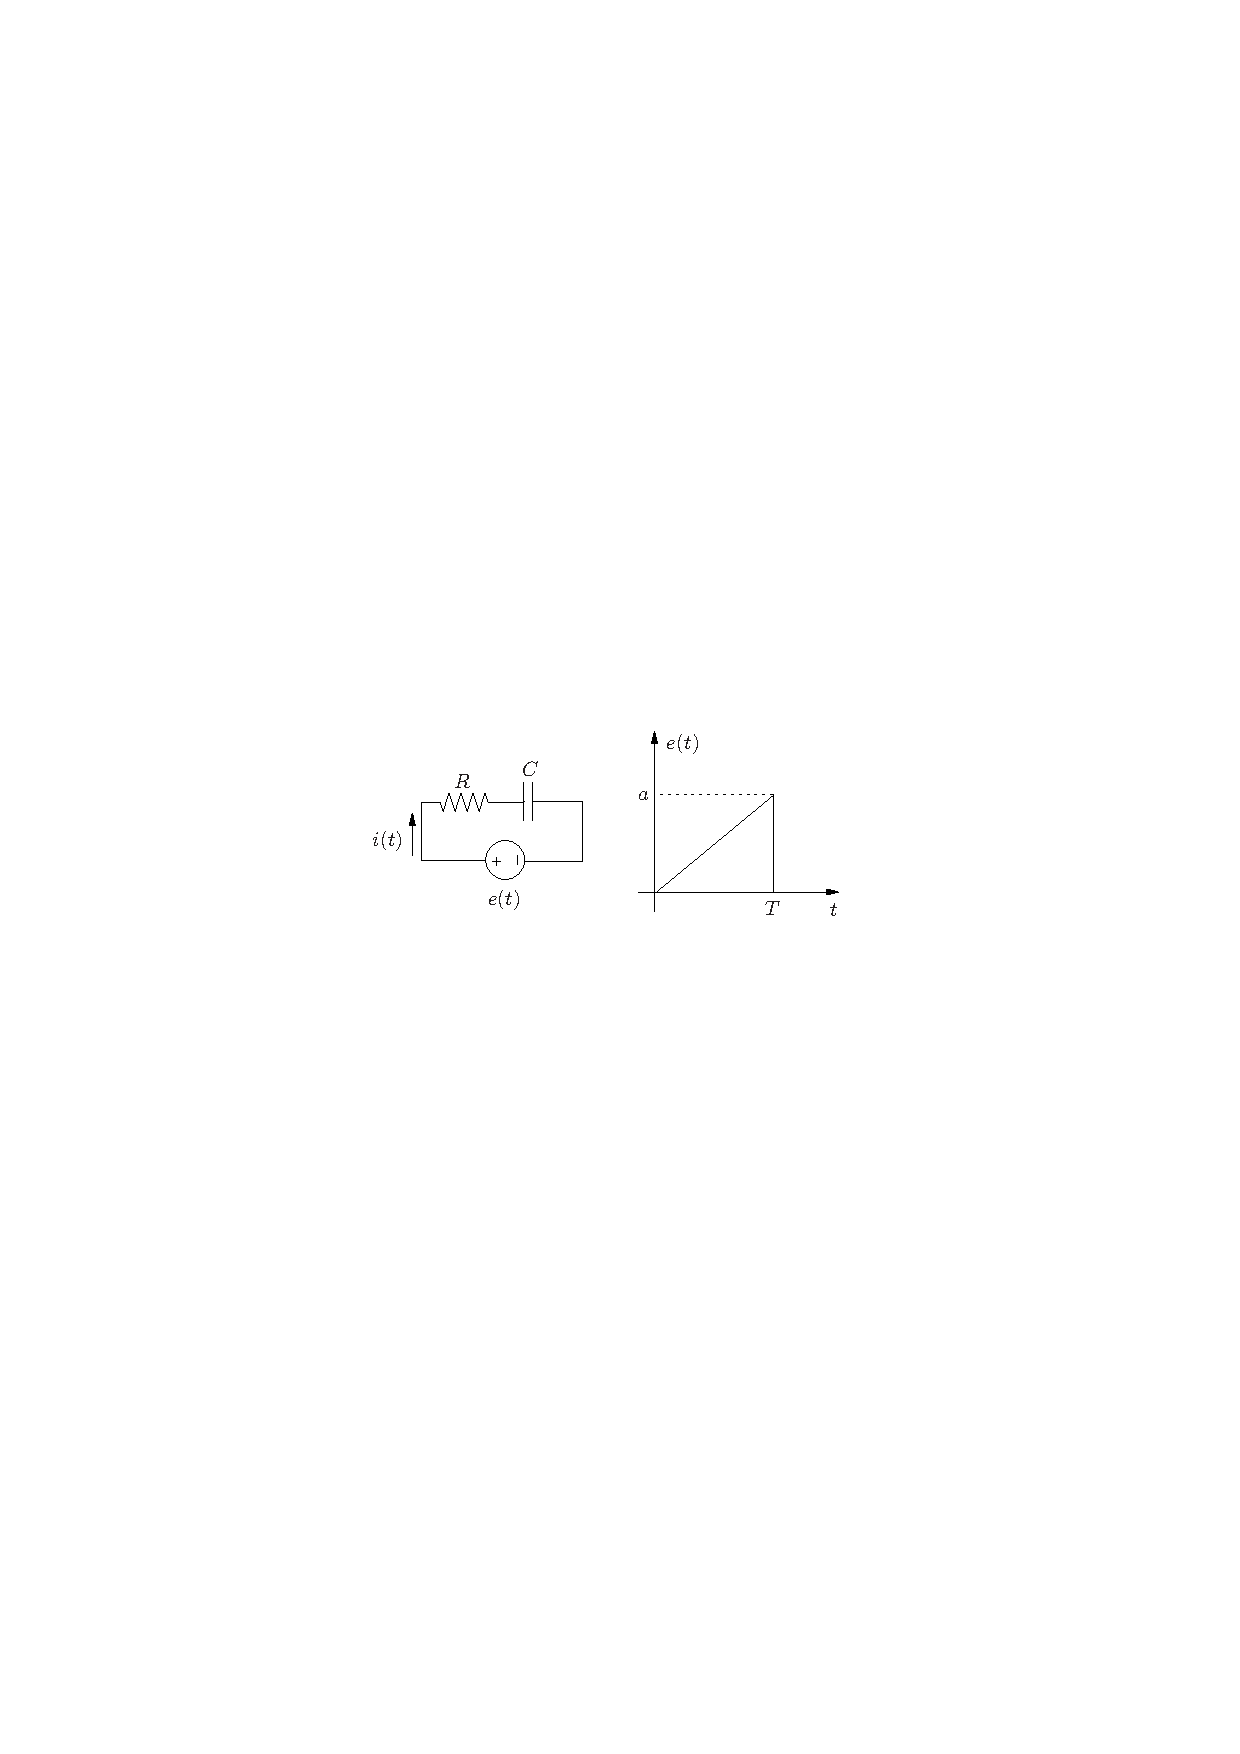
\includegraphics[width=0.7\linewidth]{exercices/ex-3-12}
\end{center}
Déterminer l'évolution du courant dans le circuit ci-dessus
lorsque la source $e(t)$ délivre le signal représenté sur la partie
droite de la figure. 

\rep{
	$i(t)= \frac{ a\tau}{ RT}(1-e^{-t/\tau})$ A, $0\leq t< T$\\
	$i(t)= e^{-t/\tau}\left(\frac{ a\tau}{ RT}(e^{T/\tau}-1)
	-\frac{ a}{ R}e^{T/\tau}\right)$ A, $t\geq T$}
\end{exercise}


\begin{exercise}{}
	\label{ex:2-13}
	\begin{center}
		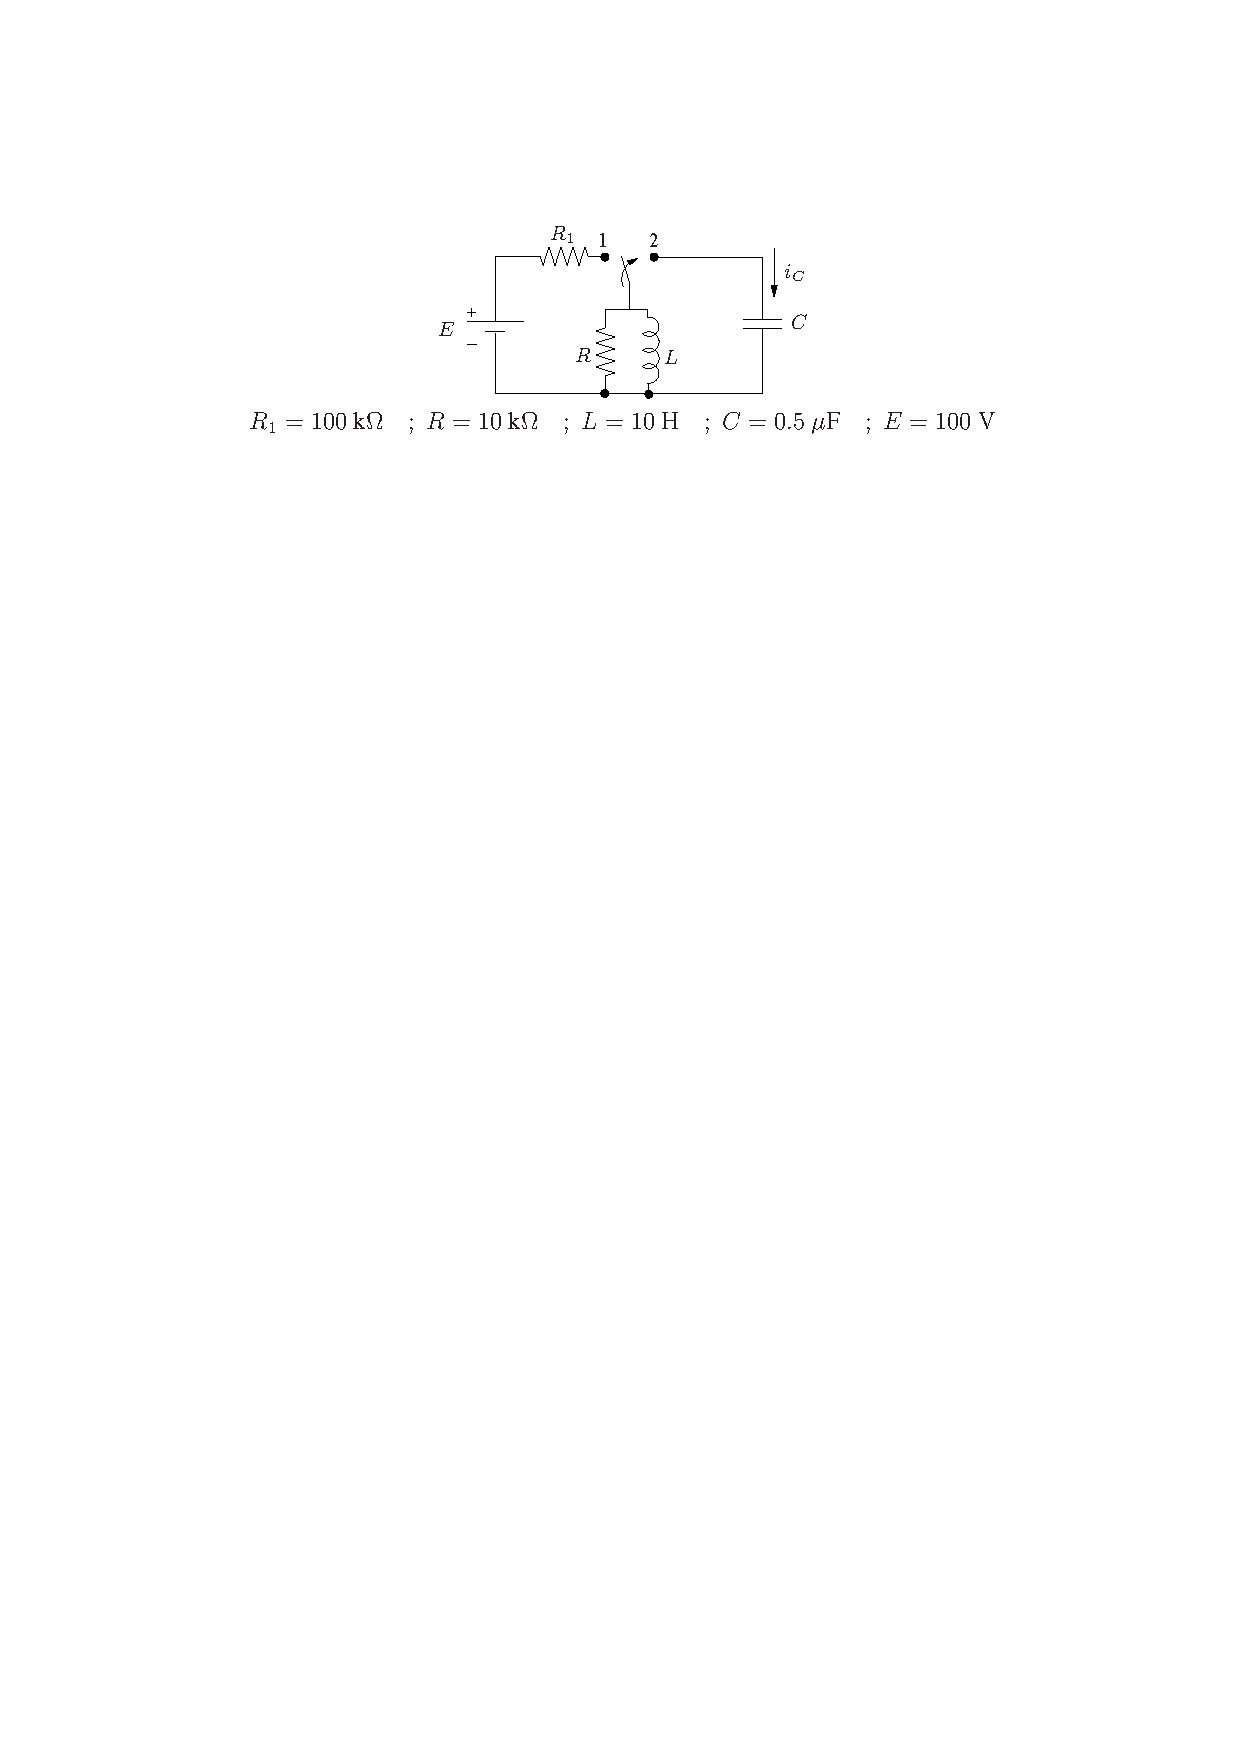
\includegraphics[width=\linewidth]{exercices/ex-3-13}
	\end{center}
	On considère le circuit ci-dessus. Durant
	l'intervalle $t<0$, l'interrupteur est en position 1 et la source
	continue $E$ est établié depuis $t=-\infty$. A l'instant $t=0$,
	l'interrupteur bascule instantanément en position 2. Déterminer
	l'évolution du courant $i_C$ parcourant le condensateur dans
	l'intervalle $t>0$. Le condensateur $C$ est supposé initialement
	relaxé.
	
	\rep{$i_C(t)=1.026\, 10^{-3}e^{-100t}\sin (436 t - 77.1^{\circ})$ V, $t\geq 0$}
\end{exercise}

\begin{exercise}{}
	\label{ex:2-15}
\begin{center}
	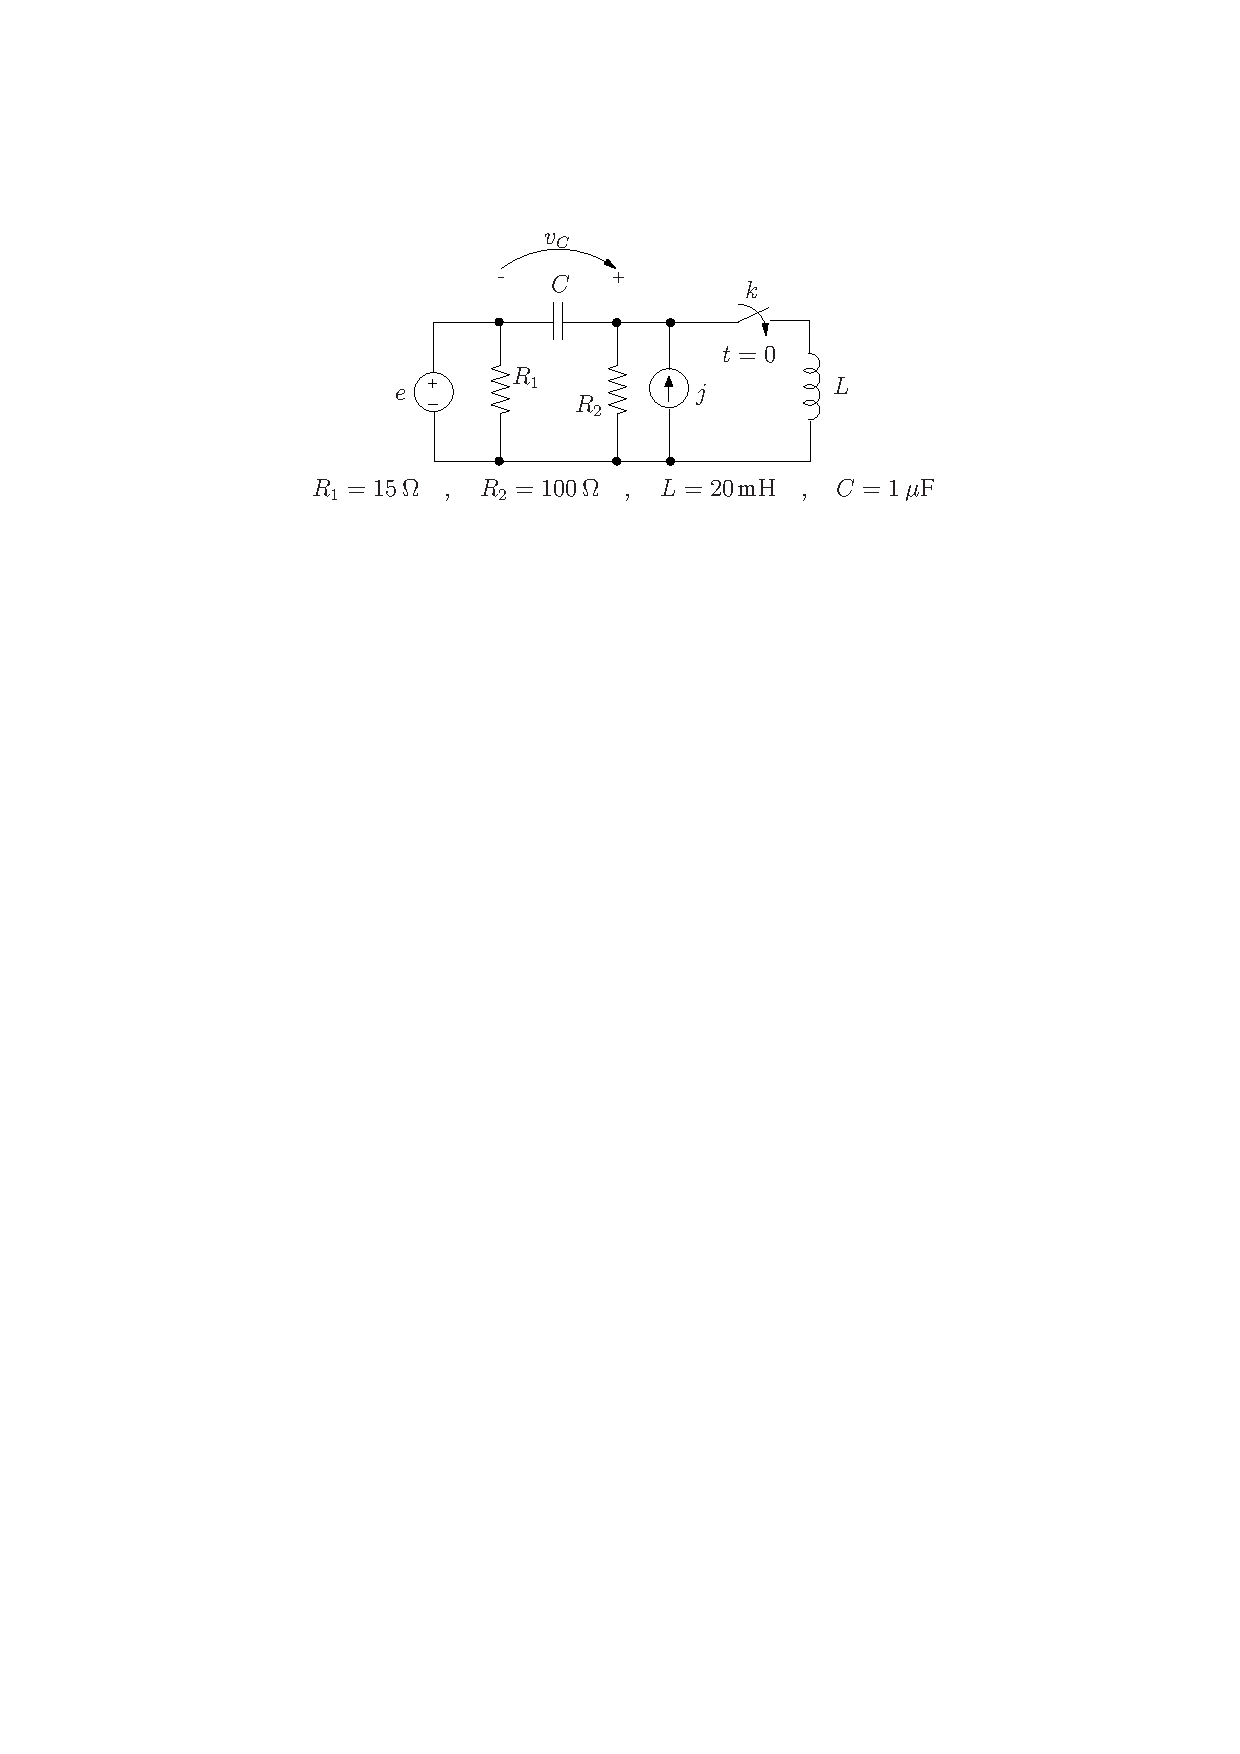
\includegraphics[width=0.7\linewidth]{exercices/ex-3-15}
\end{center}
On considère le circuit ci-dessus et les conditions de fonctionnement suivantes :
\begin{enumerate}
	\item depuis un temps supposé infini, le régime est établi avec
	l'interrupteur $k$ ouvert
	\[e = 60\,\, V \quad , \quad j= 5 \,\, A\]
	\item à l'instant $t=0$, l'interrupteur $k$ se ferme  et la f.e.m $e$
	commence à décroître selon 
	\[ e(t)=60 e^{-5t}\, ,\]
	j reste constant. L'inductance $L$ est supposée initialement relaxée.
\end{enumerate}
Questions:
\begin{enumerate}
\item Déterminer l'évolution de la tension $v_C(t)$ aux bornes du
condensateur $C$ pour $t \in [-\infty,+\infty]$.
\item Vérifier les valeurs initiale ($t=0$) et finale ($t=\infty$) de $v_C$
et justifier par un raisonnement physique. 
\item Quelles sont les fréquences naturelles du circuit ?
\end{enumerate}

\rep{$v_C(t)=440$ V, $t<0$\\
$v_C(t)= -60e^{-5t}+707.06\, e^{-5000t}\sin (5000t+\frac{\pi}{4})$ V , $t\geq 0$}
\end{exercise}


\section{Solution des exercices}
\paragraph{Exercice~\ref{ex:2-3}}~\\%
\noindent{\bf 1. Période} \ $0 \leq t \leq 15$~ms\\
L'interrupteur bascule en position $b$. 
Le condensateur est initialement non chargé~: $$v(0) = 0 \ \text{V}.$$
Le circuit se réduit à un simple circuit RC série :
\begin{center}
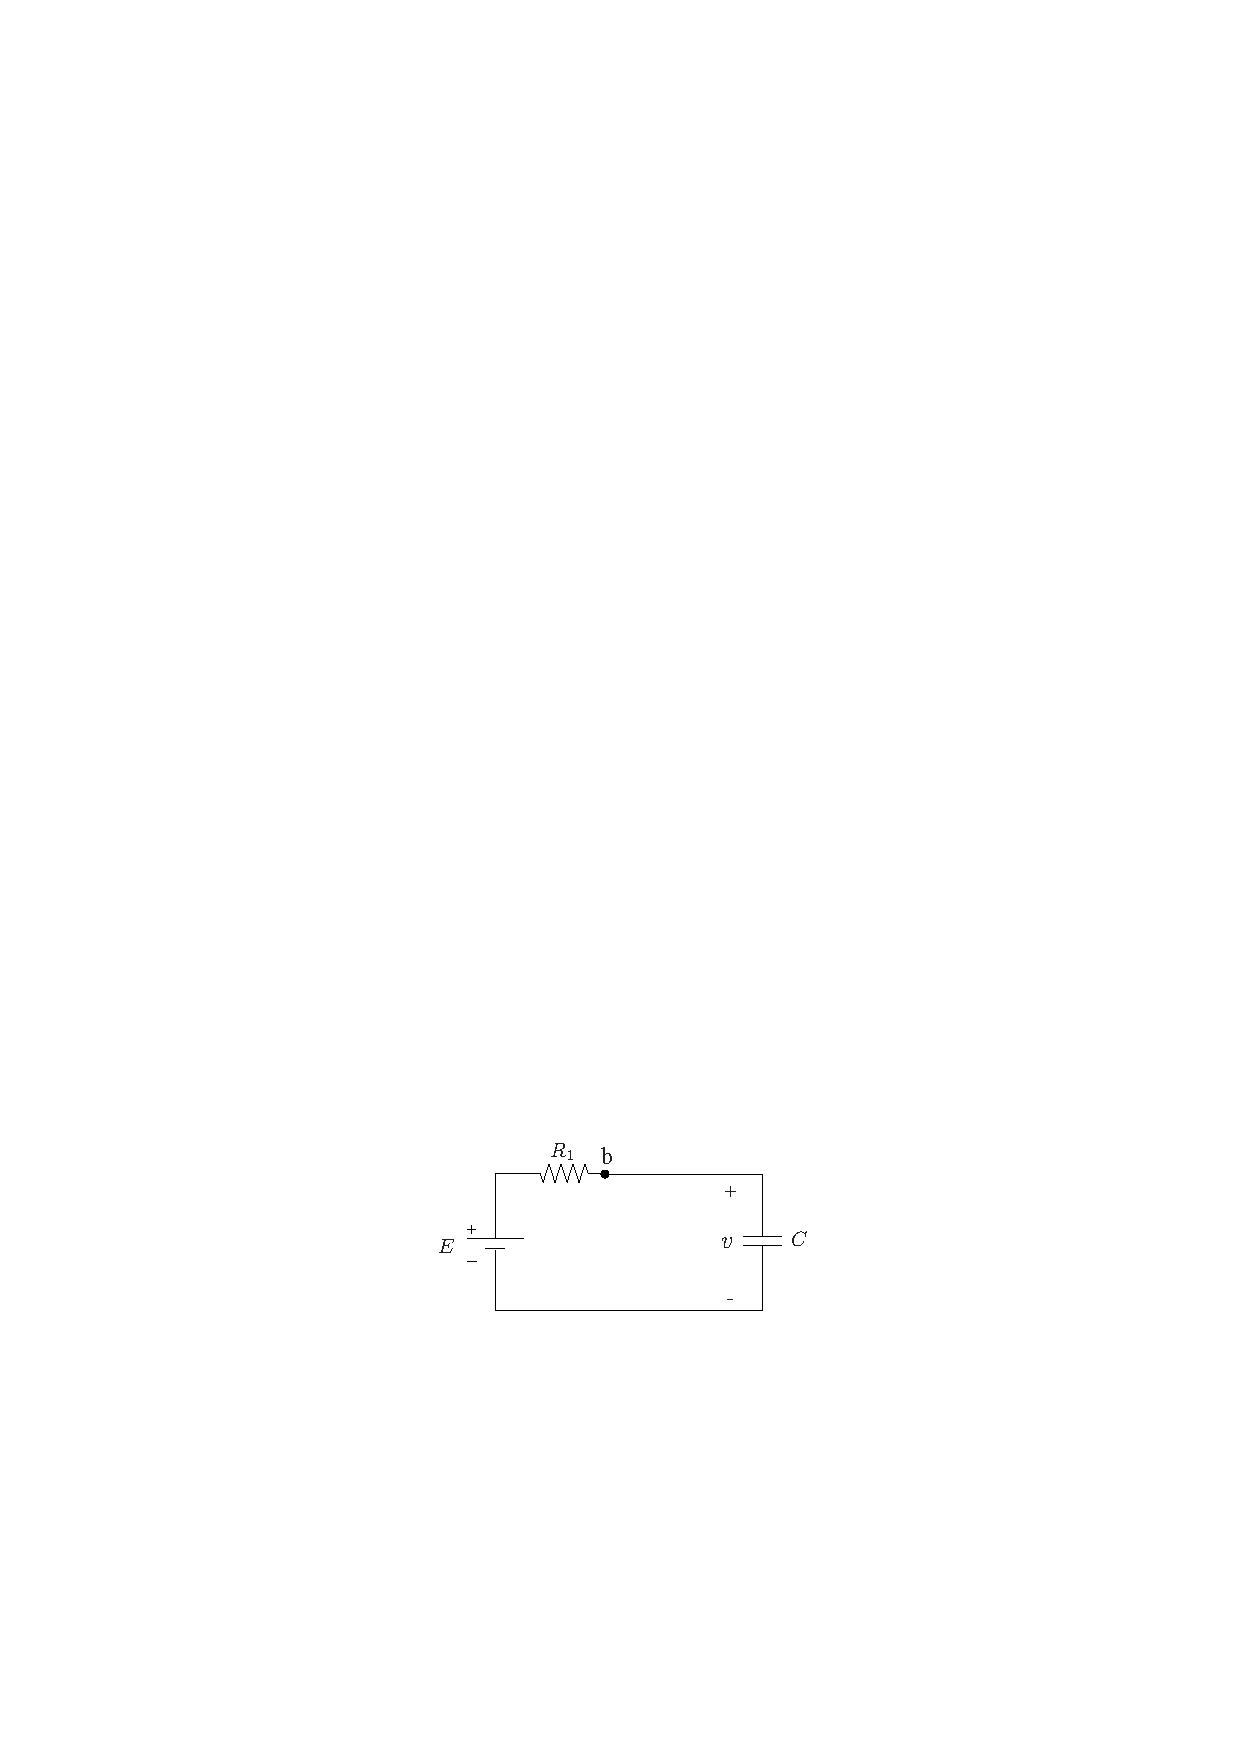
\includegraphics[width=0.55\linewidth]{sol_exercices/ex3-3-1}
\end{center}
Si on laissait l'interrupteur en position \ $b$ \ indéfiniment, le
condensateur se chargerait à la valeur de \ $E = 400\,$V~.
La constante de temps du circuit vaut~:
\[ \tau_1 \, = \, R_1C \, = \, 10^5\, . \, 10^{-7}\, 
= \, 0.01\,\mbox{s}\, = \, 10\,\mbox{ms}~. \]
L'expression de \ $v(t)$ \ est donc~:
\[ v(t) \, = \, E\, \left( 1-e^{-t/\tau_1}\right)  \, 
= \, 400\left( 1 - e^{-100t}\right) \mbox{V}~~, ~~0 \leq t \leq 15\,\mbox{ms}~. \] 
La valeur de la tension en \ $t=15\,$ms \ est~:
\[ v \left( t=15.10^{-3}\right) \, = \, 400\left( 1-e^{-1.5}\right) \, 
= \, 310.75\,\mbox{V}~. \]

\noindent{\bf Période} \ $ t \geq 15$~ms \\
L'interrupteur bascule en position \ $c$~. Le circuit devient~celui de la figure ci-dessous avec le condensateur \ $C$ \ initialement chargé à la tension \ $v_0= 310.75\,$V~.
\begin{center}
	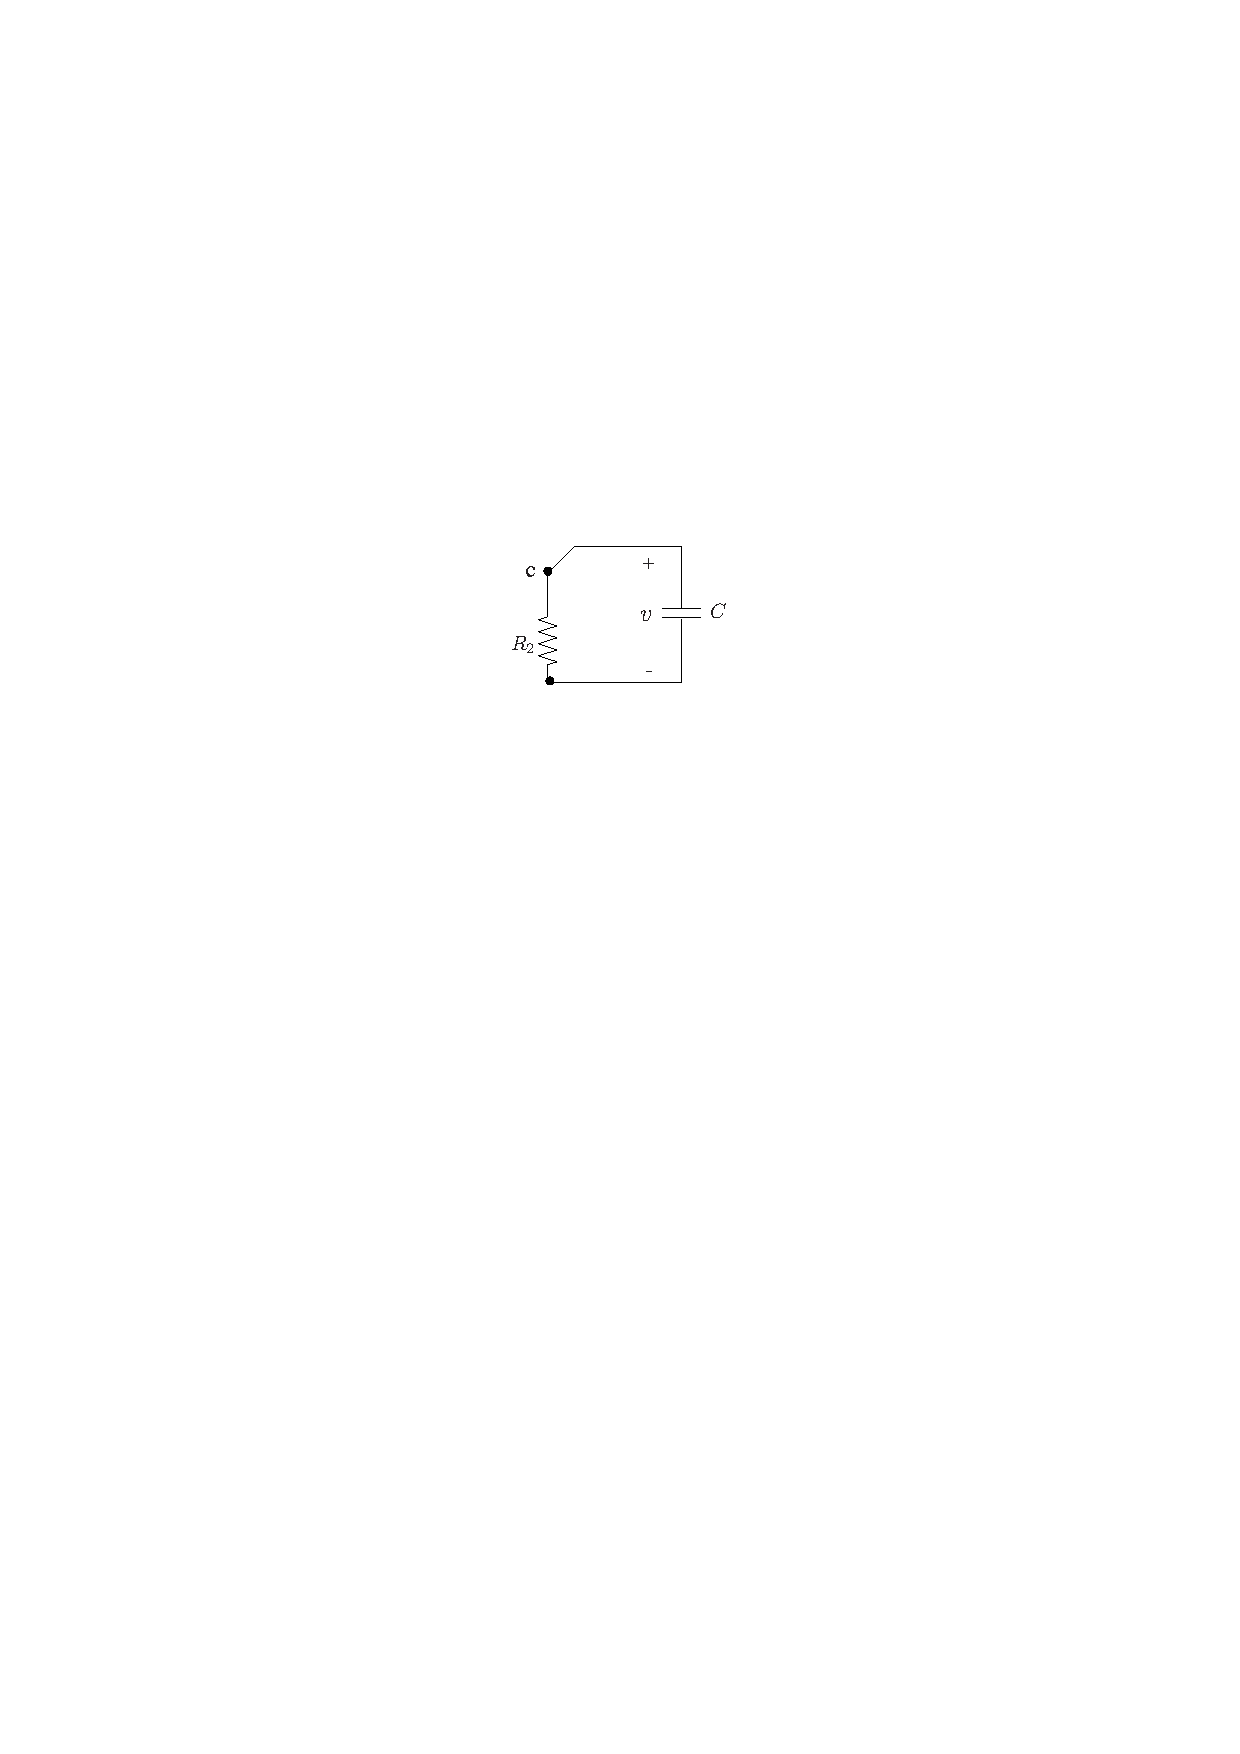
\includegraphics[width=0.35\linewidth]{sol_exercices/ex3-3-2}
\end{center}
Le condensateur se décharge dans la résistance \ $R_2$~. 
La constante de temps caractérisant cette décharge est~:
\[ \tau_2 \, = \, R_2C \, = \, 50\, 10^3\, . \, 10^{-7} \, 
= \, 0.005\,\mbox{s} \, = \, 5\,\mbox{ms}~. \]
La tension \ $v$ \  aux bornes de \ $C$ \ s'écrit alors~:
\begin{eqnarray*}
	v(t) &=& v_0 \, e^{-(t-0.015)/\tau_2}\\
	&=& 310.75\, e^{-200(t-0.015)}~~,~~t \geq 15\,\mbox{ms}~.
\end{eqnarray*}

Remarquons qu'il importe de changer l'origine des temps dans
l'expression de \ $v$~; la valeur initiale \ $v_0 = 310.75$ \ se
produisant à l'instant \ $t=15\,$ms~. On remplace donc dans
l'expression générale de la tension de décharge du condensateur \ $t$
\ par \ $t'=t-0.015$~.

\noindent{\bf 2. Tracé de \ $ v(t)$}
\begin{center}
	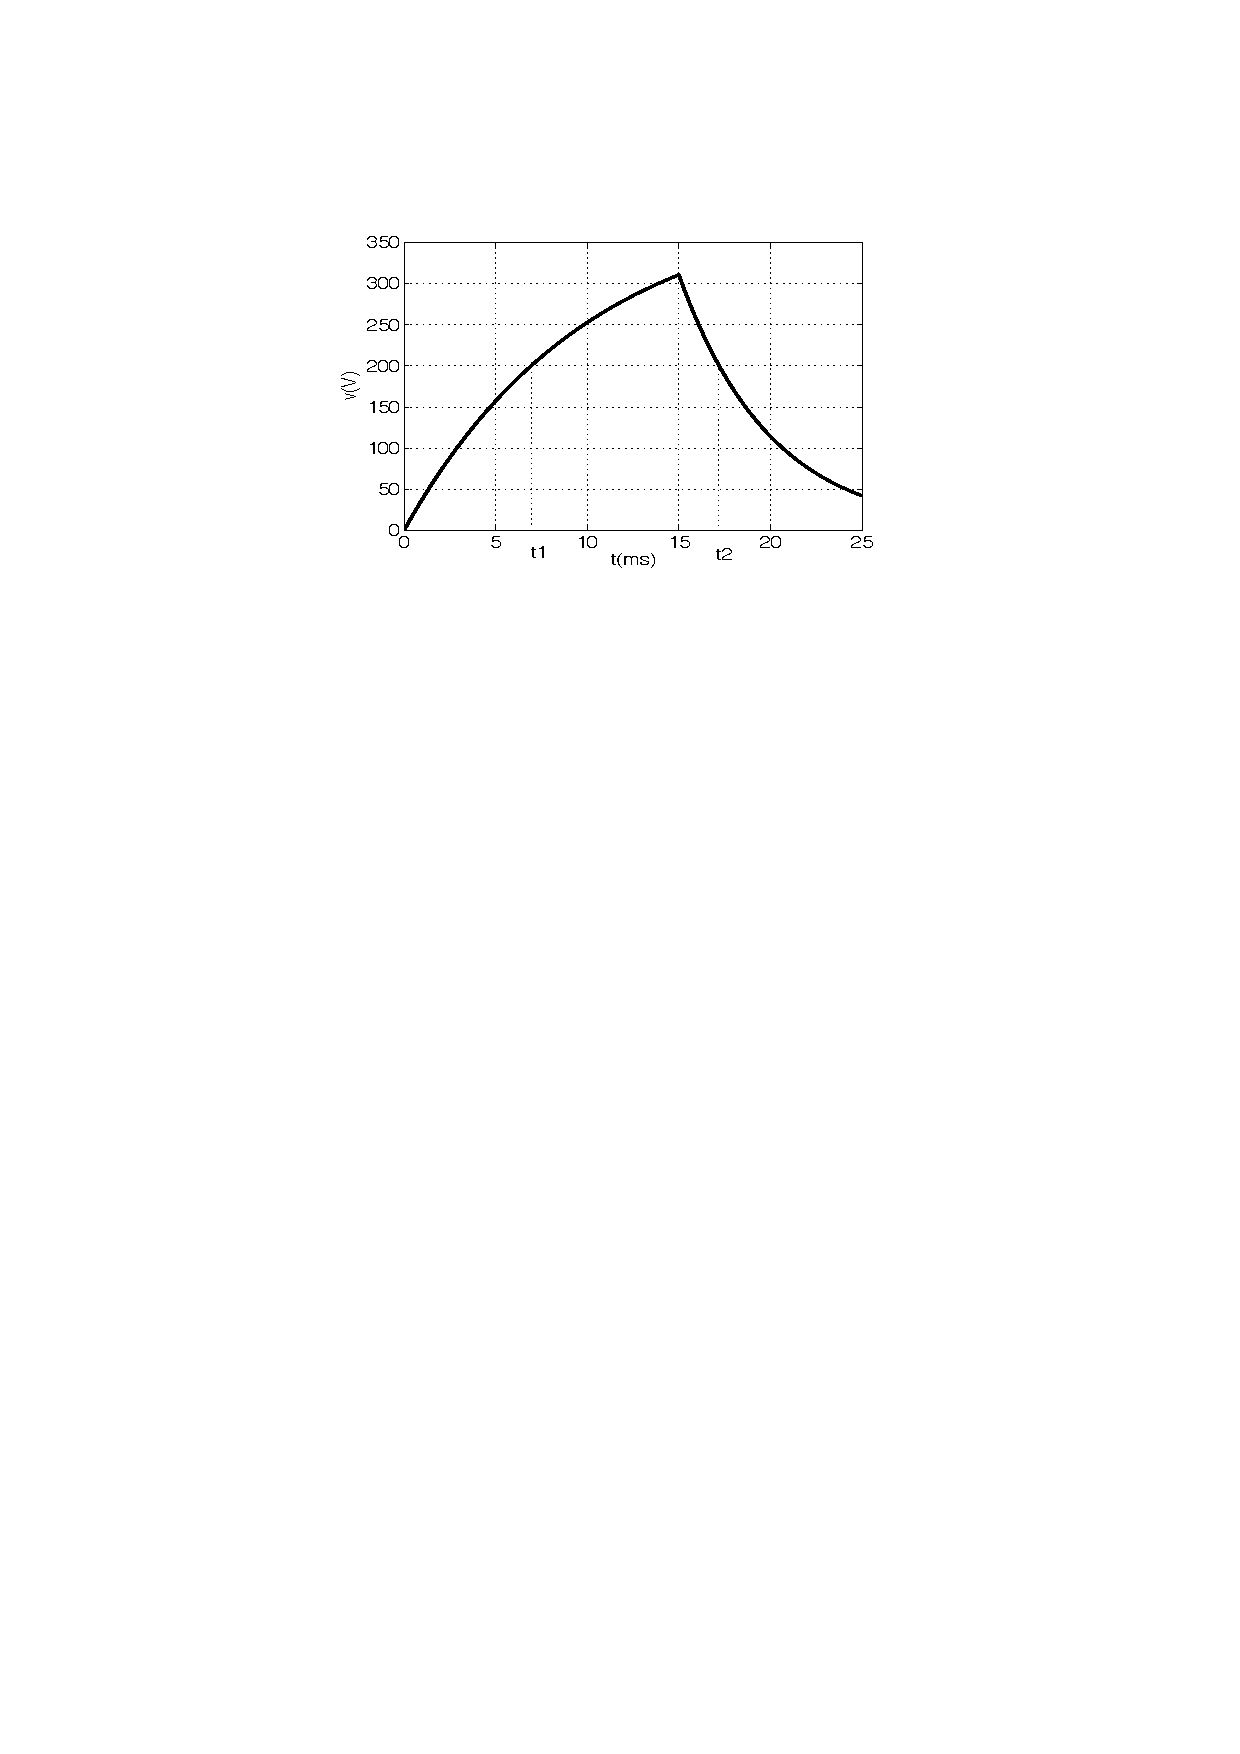
\includegraphics[width=0.6\linewidth]{sol_exercices/ex3-3-3}
\end{center}

\noindent{\bf 3. Instants auxquels \ $v = 200\,$V}\\
D'après le tracé de $ v(t)$, on remarque que \ $v$ \
atteint 200$\,$V à la fois dans la période de charge \ $(0 \leq t \leq
0.015)$ \ et dans la période de décharge \ $(t \geq 0.015)$~.

\begin{enumerate}
	\item période de charge~: il faut
	\begin{eqnarray*}
		400 - 400\, e^{-100t_1} &=& 200\\
		e^{-100t_1} &=& 0.5\\
		t_1 &=& \dfrac{ \mbox{ln}\, 0.5}{-100} \: = \: 6.93\,\mbox{ms}
	\end{eqnarray*}
	\item période de décharge~: il faut
	\begin{eqnarray*}
		310.75\, e^{-200(t_2-0.015)} &=& 200\\
		e^{-200t_2} &=& \dfrac{200}{310.75\, e^3} \: = \: 0.03204\\
		t_2 &=& 17.2\,\mbox{ms}~.
	\end{eqnarray*}
\end{enumerate}

\paragraph{Exercice~\ref{ex:2-5}}~\\%
On recherche la réponse libre avec les conditions initiales~:
\begin{eqnarray*}
	u_1(0) &=& u_{10} \: = \: 2\, \mbox{V}\\
	u_2(0) &=& u_{20} \: = \: 5\, \mbox{V}
\end{eqnarray*}
comme indiqué à la figure suivante :
\begin{center}
	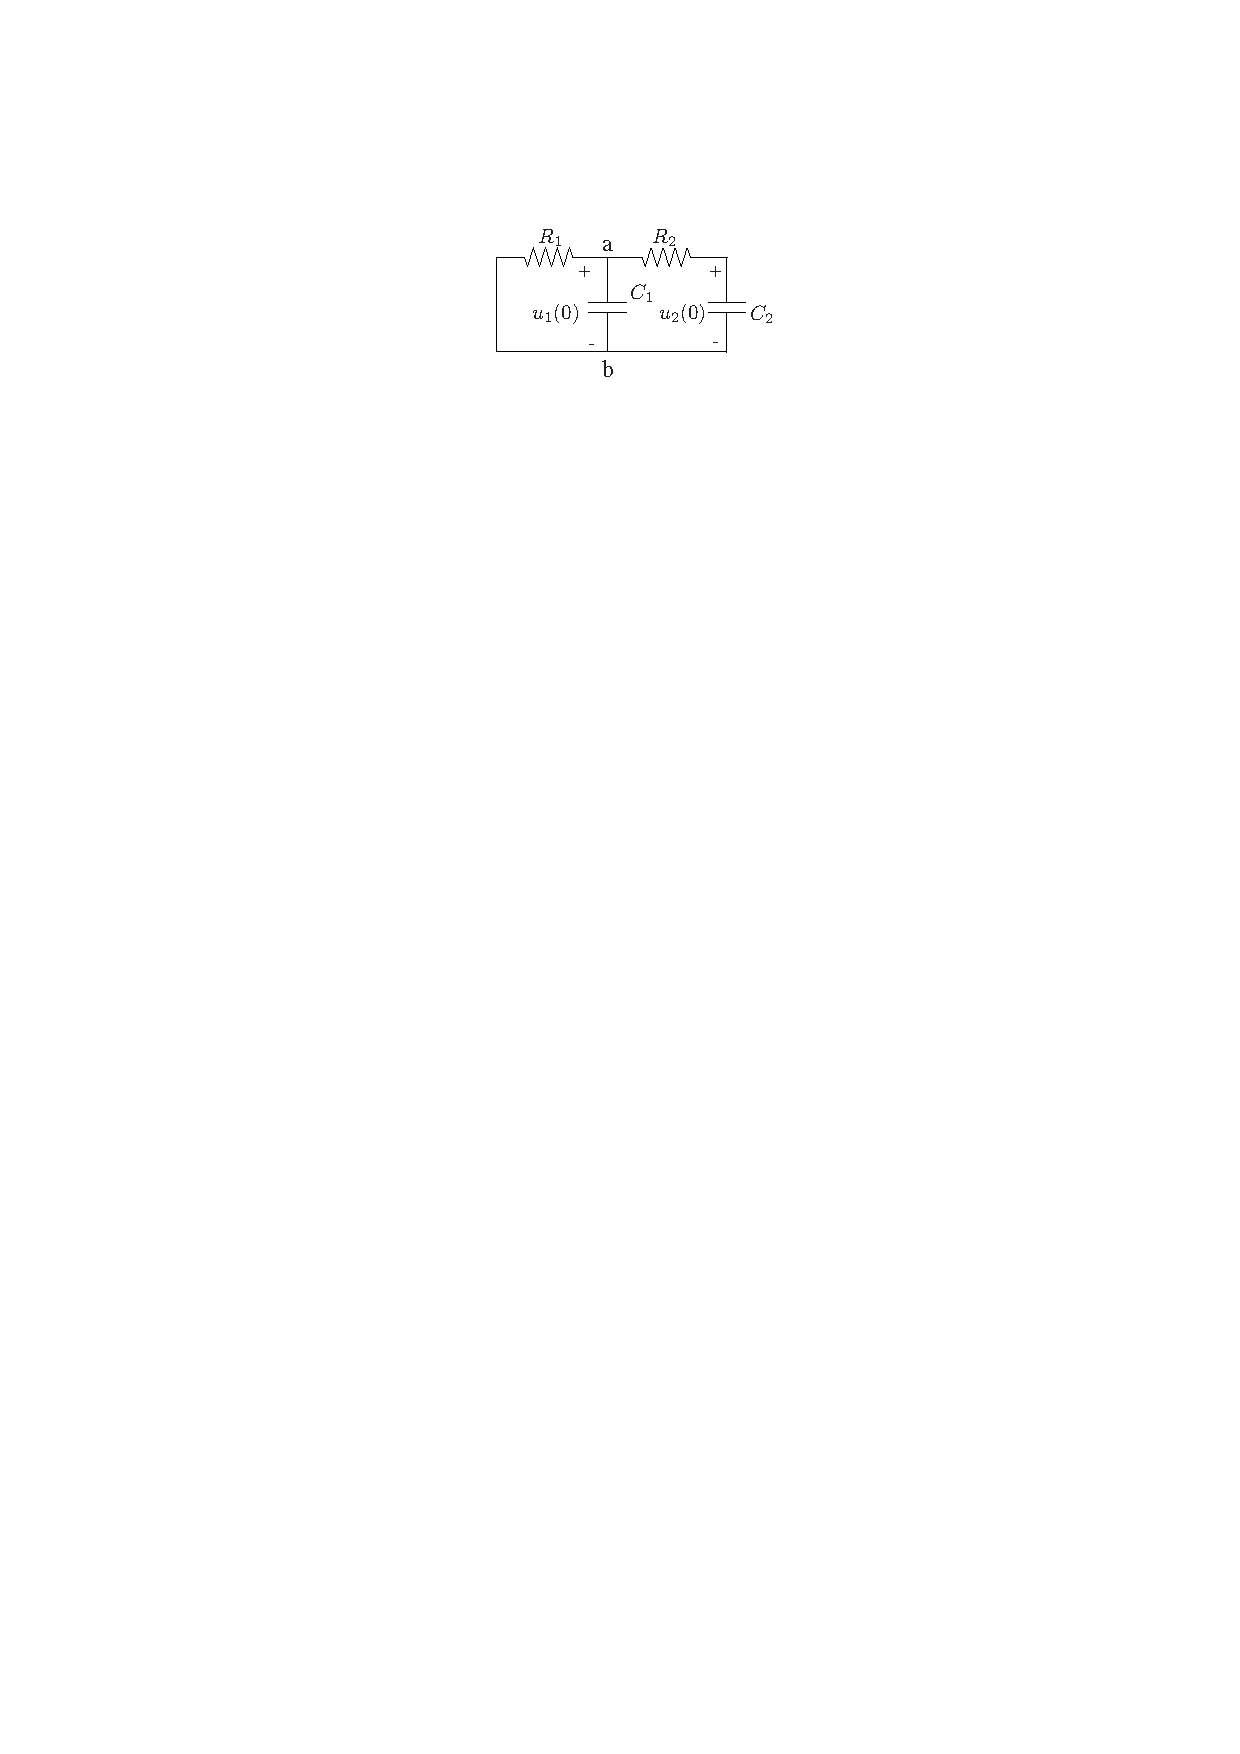
\includegraphics[width=\linewidth]{sol_exercices/ex3-5}
\end{center}
La PLK écrite aux noeuds \ $a$ et $b$ \ fournit~:
\begin{eqnarray}
C_1 \, \dfrac{du_1}{dt} + \dfrac{u_1}{R_1} + \dfrac{u_1-u_2}{R_2} 
&=& 0 \label{1}\\C_2 \, \dfrac{du_2}{dt} +  \dfrac{u_2-u_1}{R_2} &=& 0 \label{2}
\end{eqnarray}
Il faut résoudre cet ensemble de 2 équations différentielles à 2
inconnues \ $u_1$ et $u_2$~.
De (\ref{2}), on tire~:
\begin{equation}
u_1 \: = \: R_2C_2 \, \dfrac{du_2}{dt} + u_2~.\label{3}
\end{equation}
Rempla\c{c}ant dans (\ref{1}), on déduit l'équation différentielle
pour \ $u_2$~:
\[ \dfrac{d^2u_2}{dt^2} + \left( \dfrac{1}{R_2C_2} + \dfrac{1}{R_2C_1} 
+ \dfrac{1}{R_1C_1} \right) \dfrac{du_2}{dt} +
\dfrac{u_2}{R_1R_2C_1C_2} \: = \: 0~. \] La solution générale de cette
équation différentielle à coefficients constants s'écrit~:
\[ u_2(t) \: = \: K_1\, e^{s_1t} + K_2\, e^{s_2t} \]
avec \ $s_1\, , \, s_2$ \ les solutions de l'équation caractéristique~:
\[ s^2 + \left( \dfrac{1}{R_2C_2} + \dfrac{1}{R_2C_1} + \dfrac{1}{R_1C_1} \right) s
+ \frac{1}{R_1R_2C_1C_2}=0~. \]
Le discriminant de cette équation est~:
\[  \Delta \: = \: \left( \dfrac{1}{R_2C_2} + \dfrac{1}{R_2C_1} 
+ \dfrac{1}{R_1C_1} \right)^2 - \dfrac{4}{R_1R_2C_1C_2}~. \]
Il peut aussi s'écrire~:
\[  \Delta \: = \: \left( \dfrac{1}{R_2C_2} + \dfrac{1}{R_2C_1} 
- \dfrac{1}{R_1C_1} \right)^2 + \dfrac{4}{R_1R_2C_1^2}\: > \ 0~. \] On
remarque que ce discriminant ne peut être négatif. Les solutions de
l'équation caractéristique sont donc 2 nombres réels quelles que
soient les valeurs des éléments \ $R_1,R_2$, $C_1,C_2$~. La réponse libre
de tout circuit RC est donc toujours de type apériodique; elle ne peut
être de forme oscillante.

Les racines de l'équation caractéristique, ou fréquences naturelles du
circuit, sont donc~:
\[ s_{1,2} \: = \, -\, \dfrac{1}{2} \left( \dfrac{1}{R_2C_2} + \dfrac{1}{R_1C_1} 
+ \dfrac{1}{R_1C_1} \right) \pm \sqrt{\,\dfrac{\Delta}{4}~}~. \] On
remarque que lorsque les éléments sont passifs \ $(R_1,R_2,C_1,C_2 >
0)$~, ces racines sont 2 nombres négatifs, la réponse libre s'atténue
donc avec le temps (circuit stable).

Rempla\c{c}ant par les valeurs numériques, on trouve~:
\[ s_1 = -0.63~~~~~\mbox{et}~~~~~s_2 = -6.37~.\]

De (\ref{3}), on déduit l'expression de la tension \ $u_1$~:
\begin{eqnarray*}
	u_1 &=& (R_2C_2s_1+1) \, K_1\, e^{-0.63t} + (R_2C_2s_2+1) \, K_2 \, e^{s_2t} \\
	&=& 0.84\, K_1 \, e^{-0.63t} - 0.59\, K_2\, e^{-6.37t}~. 
\end{eqnarray*}
Les constantes \ $K_1$ et $K_2$ \ se déduisent des conditions innitiales pour \ $u_1$ et $u_2$~.
On a~:
\begin{eqnarray*}
	u_1(0) &=& u_{10} \: = \: 2 \: = \: 0.84\, K_1 - 0.59\, K_2\\
	u_2(0) &=& u_{20} \: = \: 5 \: = \: K_1 + K_2~.
\end{eqnarray*}
On trouve~:
\[ K_1 = 3.46 ~~~~~\mbox{et}~~~~~K_2 = 1.54~. \]
Finalement, les expressions de \ $u_1$ et $u_2$ \ sont~:
\begin{eqnarray*}
	u_1(t) &=& 2.9\, e^{-0.63t} - 0.91 \, e^{-6.37t}\mbox{~V}\\
	u_2(t) &=& 3.46\, e^{-0.63t} - 1.54 \, e^{-6.37t}\mbox{~V~.}
\end{eqnarray*}

\paragraph{Exercice~\ref{ex:2-6}}~\\%
De l'expression de \ $v(t)$~:
\[ v(t) \: = \: D_1\, t\, e^{-4000t} + D_2\, e^{-4000t}~~, ~~t\geq 0~, \]
on déduit que~:
\begin{enumerate}
	\item le régime est un régime apériodique critique
	\item l'équation caractéristique relative à l'équation différentielle
	qui caractérise \ $v$ \ admet une racine double~:
	\[ s_1 \, = -4000~. \]
\end{enumerate}
Recherchons cette équation différentielle.
La PLK écrite pour le circuit de la ci-dessous fournit~:
\[ \begin{array}{c}
i_R + i_L + i_C \, = \, 0\\[3mm]
\dfrac{v}{R} + {\displaystyle \frac{1}{L}} {\displaystyle \int^t_0} v(x) \, dx 
+ i_0 + C\, {\displaystyle \frac{dv}{dt}} \: = \: 0\end{array} \]
\begin{center}
	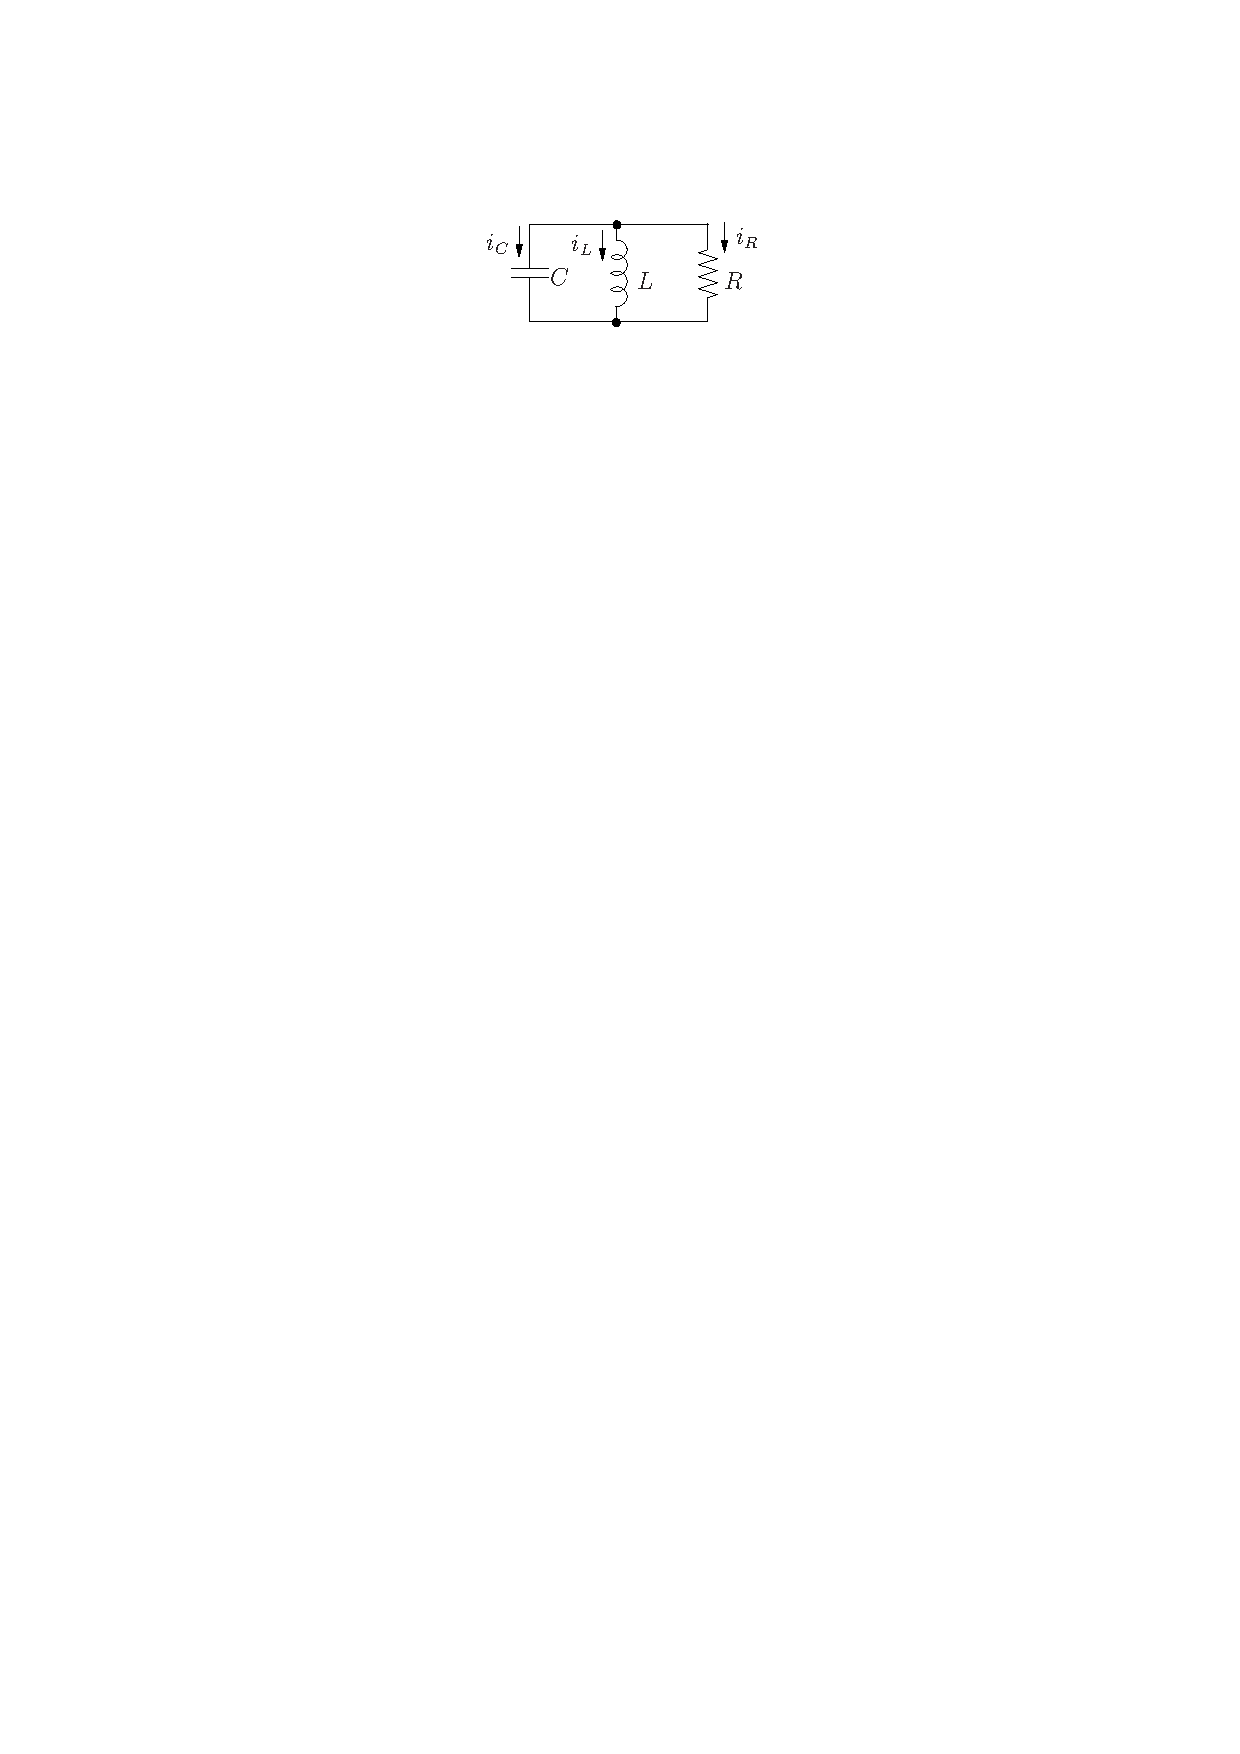
\includegraphics[width=\linewidth]{sol_exercices/ex3-6}
\end{center}

Dérivant cette relation, on trouve~:
\[ \dfrac{d^2v}{dt^2} + \dfrac{1}{RC} \, \dfrac{dv}{dt} + \dfrac{1}{LC} \, v \: = \: 0~. \]
L'équation caractéristique correspondante est~:
\[ s^2 + \dfrac{1}{RC} \, s + \dfrac{1}{LC} \: = \: 0~. \]
Ses racines peuvent se mettre sous la forme~:
\[ s_{1,2} \: = \, -\alpha \pm \sqrt{\alpha^2 - \omega_0^2\,} \]
avec
\begin{eqnarray*}
	\alpha &=& \dfrac{1}{2RC}~, ~~\mbox{le coefficent d'amortissement}\\
	\omega_0 &=& \dfrac{1}{\, \sqrt{LC}\,}~, ~~\mbox{la fréquence de résonance du circuit.}
\end{eqnarray*}
Dans le cas considéré ici, nous avons~:
\[ s_1 \, =\,  s_2\, =\,  -\alpha~. \]
soit
\[ 4000 \, =\,  \dfrac{1}{2RC}~. \]
Nous savons que le discriminant de l'équation caractéristique est nul et donc que~:
\[ \alpha^2 - \omega_0^2 \, = \, \left( \dfrac{1}{2RC}\right)^2 - \dfrac{1}{LC} \, = \, 0 \]
ou en rempla\c{c}ant les valeurs numériques connues~:
\[  (4000)^2 - \dfrac{1}{5C} \: = \: 0~. \]
On déduit la valeur de la capacité~:
\[ C \: = \: \dfrac{1}{5.(4000)^2} \: = \: 12.5\, \mbox{nF~} \]
et comme
\[ \dfrac{1}{2RC} \, = \, 4000~,\]
on déduit la valeur de la résistance
\[ R \: = \: \dfrac{1}{2\: . \: 12.5\, 10^9\, . \, 4000} \: = \: 10\,\mbox{k}\Omega~. \]
Les conditions initiales fournissent~:
\[ v(0) \, = \, v_0 \, = \, \left. v(t)\right|_{t=0} \,=  D_2~. \]
Dès lors,
\[ D_2 \, = \, 25\, \mbox{V}~. \]
D'autre part, la continuité du courant dans l'inductance impose~:
\[ i_L(^+) \, = \, i_L(0^-) \, = \, i_0 \, = \, 5\, \mbox{mA}~.\]
Or
\[ i_C(0^+) \, = -\, i_R(0^+) - i_L(0^+) \]
avec
\begin{eqnarray*}
	i_C(0^+) &=& C \left. \frac{dv}{dt}\right|_{t=0} \, = \: C\left( D_1 - 4000\, D_2 \right)\\
	i_R(0^+) &=& \frac{v_0}{R}\\
	i_L(0^+) &=& i_0\\
	D_1 &=& -\, \frac{v_0}{RC} - \frac{i_0}{C} + 4000\, v_0\\
	&=& -\, 5\, 10^5
\end{eqnarray*}
et finalement
\[ v(t) \: = \, -\, 3.2\, 10^5\, t \, e^{-4000t} + 25\, e^{-4000t}~. \]

\paragraph{Exercice~\ref{ex:2-7}}~\\%
\noindent{\bf 1. Période \ $t<0$}\\
Le circuit considéré se réduit à
\begin{center}
	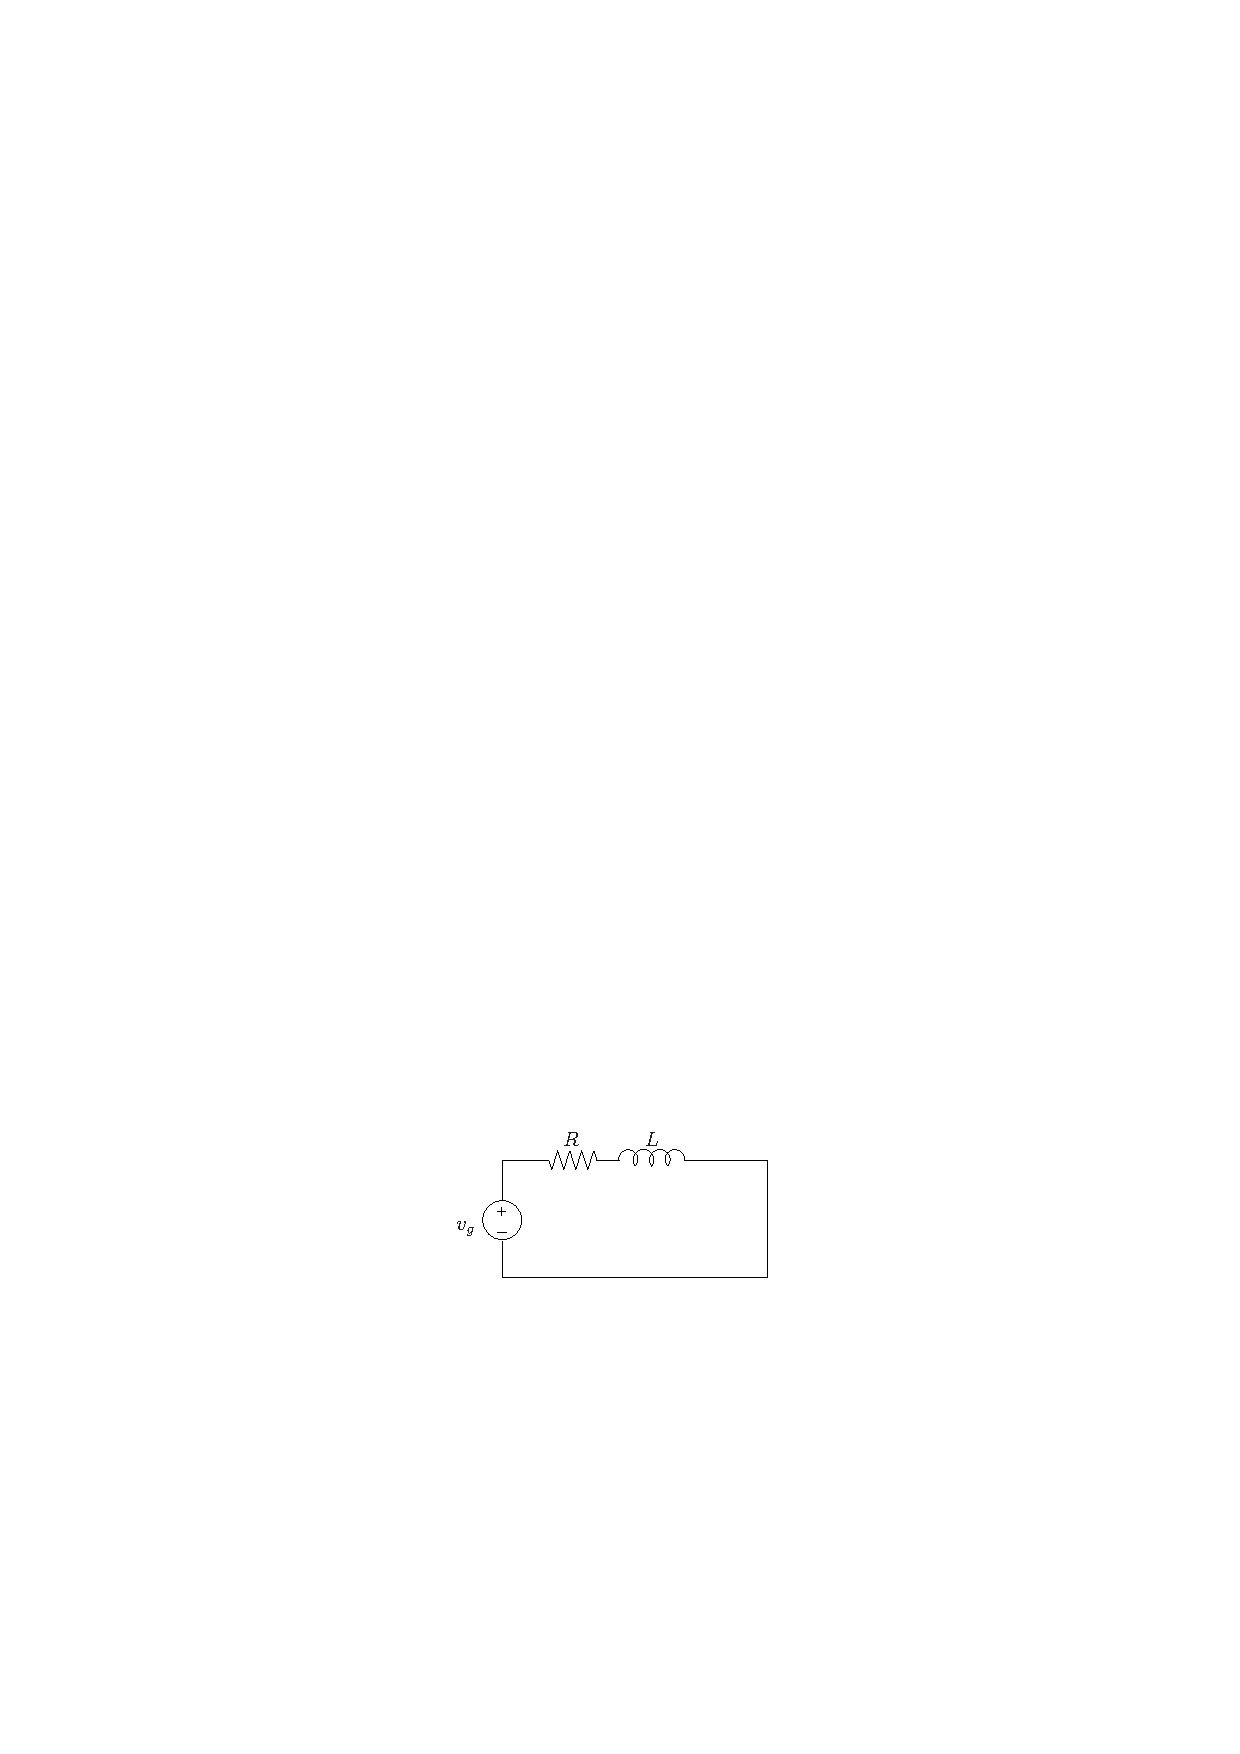
\includegraphics[width=\linewidth]{sol_exercices/ex3-7-1}
\end{center}
Le régime est établi et l'inductance est parcourue par un courant~:
\[ i_{L0} \, = \, \dfrac{v_g}{R}~. \]
La tension à ses bornes est nulle.

\noindent{\bf 2. Période \ $t\geq 0$}\\
Le circuit devient
\begin{center}
	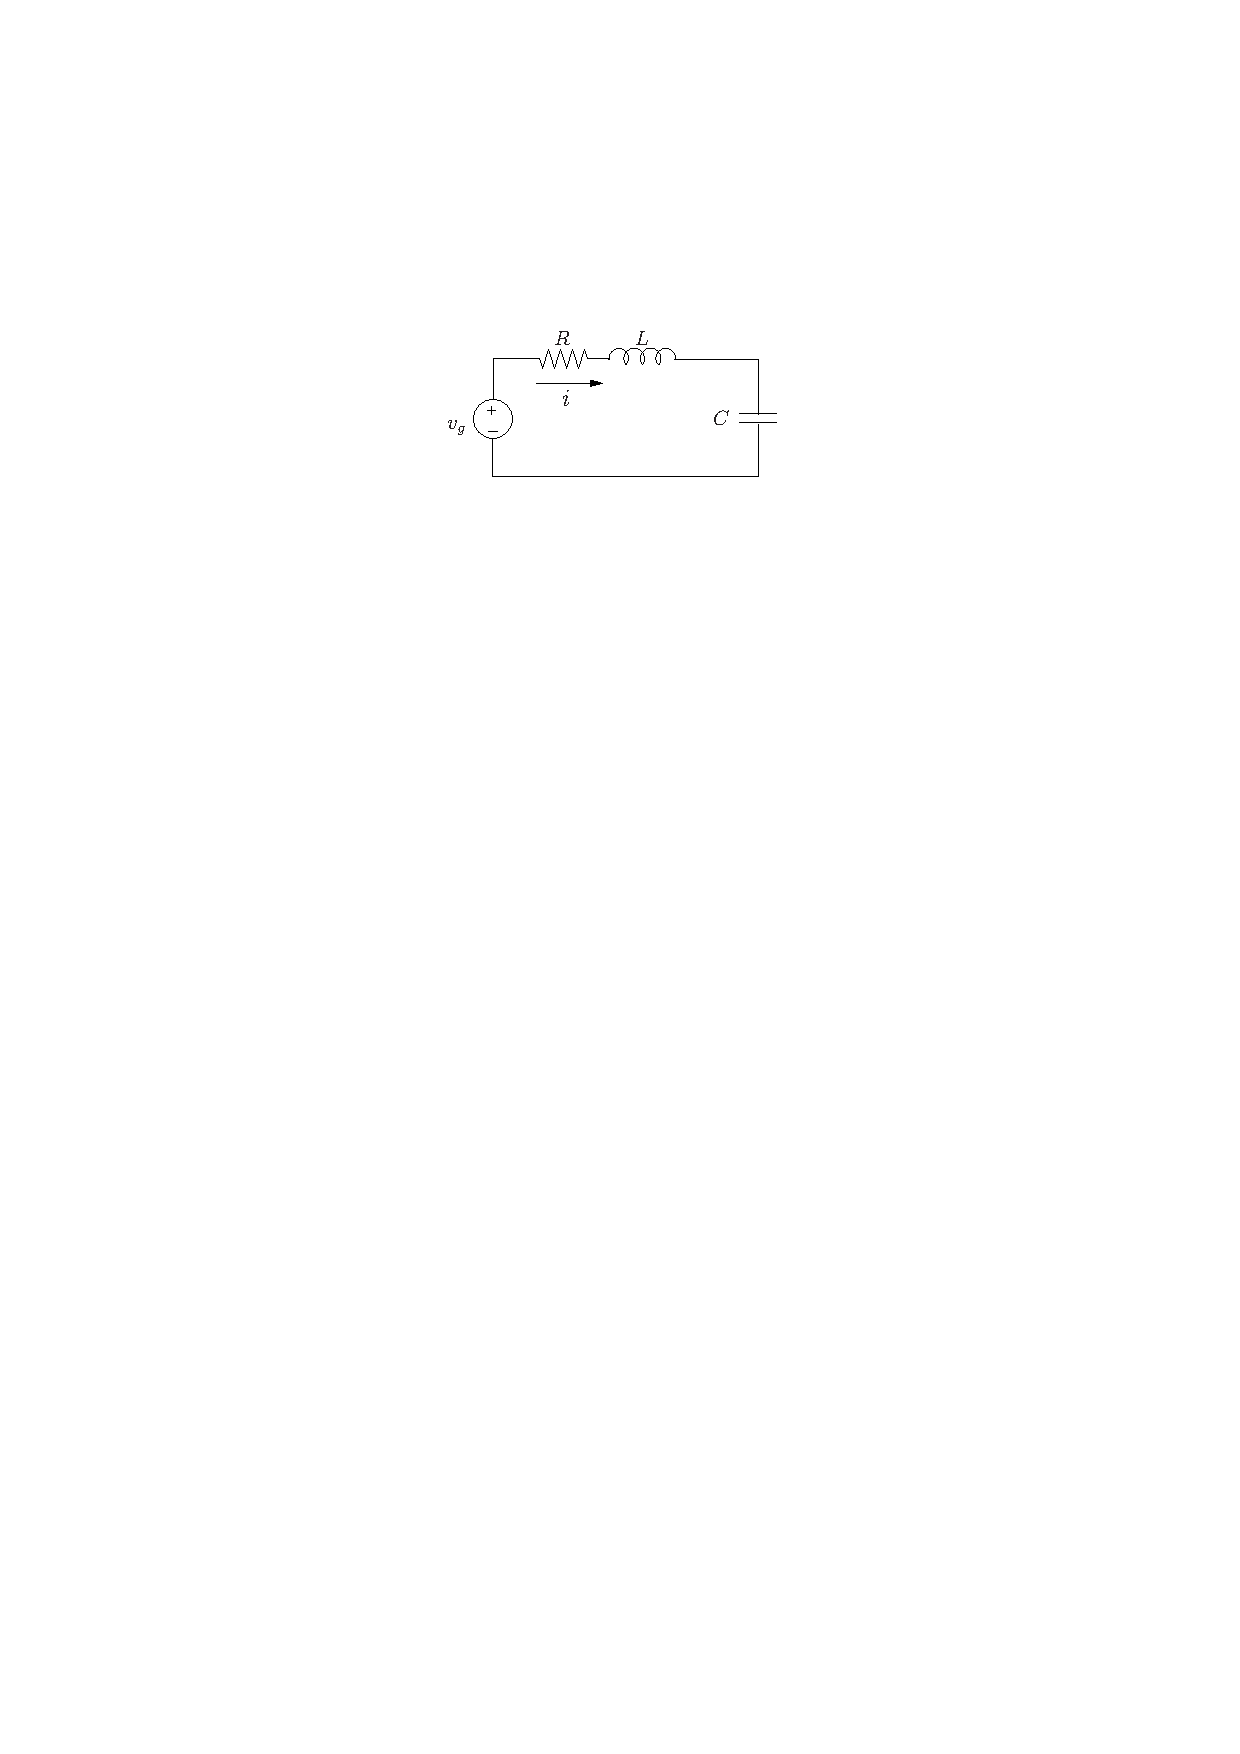
\includegraphics[width=\linewidth]{sol_exercices/ex3-7-2}
\end{center}
Les conditions initiales sont~:
\begin{eqnarray*}
	v_{C0} &=& 0\\
	i_{L0} &=& \frac{v_g}{R}~.
\end{eqnarray*}
La réponse du circuit est oscillatoire amortie. Le courant \ $i$ \
parcourant le circuit peut donc s'écrire~:
\[ i(t) \: = \: A \, e^{-\alpha t} \cos\, \omega_d t + 
B\, e^{-\alpha t} \sin \, \omega_d t\, \text{A~}, ~~t\geq 0 \]
avec \ $\alpha$~, l'amortissement, égal à \ $R/2L$
et \ $\omega_d$~, la fréquence d'oscillation.

Les constantes \ $A$ et $B$ \ sont fixées par les conditions initiales~:
\begin{eqnarray*}
	i(t=0) &=& i_{L_0} \: = \: \frac{v_g}{R}\: = \: A\\
	v_C(t=0) &=& 0~.
\end{eqnarray*}
Par application de la SLK, on écrit~:
\[ v_C(t) \: = \: v_g - Ri - L\dfrac{di}{dt}~. \]
En \ $t=0$~, on a~:
\[ v_g \: = \: Ri + L\dfrac{di}{dt} \]
soit
\begin{eqnarray*}
	v_g &=& RA - A\alpha L + BL\omega_d\\
	&=& v_g - \frac{v_g}{R} \, \alpha L + BL\omega_d~.
\end{eqnarray*}
On déduit~:
\[ B \: = \: \dfrac{v_g}{R} \, . \, \dfrac{R}
{2L} \, . \,L \, . \, \dfrac{1}{L\omega_d} \: = \: \dfrac{v_g}{2L\omega_d} \] 
et
\[ i(t) \: = \: \dfrac{v_g}{R} e^{-\alpha t}  \cos \, \omega_d t \,  +
\dfrac{v_g}{2L\omega_d} \:  e^{-\alpha t}  \sin \, \omega_d t ~\mbox{A}~, ~t\geq 0~. \]
On déduit finalement l'expression de \ $v_0(t)$~:
\begin{eqnarray*}
	v_0(t) &=& L \, \dfrac{di}{dt}\\[2mm]
	&=& -\, \dfrac{v_g}{R} \, . \, \dfrac{R}{2L} \, . \, L e^{-\alpha t} \cos \, \omega_d t 
	- \dfrac{v_g}{R} \, L\omega_d \, e^{-\alpha t} \sin \, \omega_d t\\[2mm]
	&&- \dfrac{v_g}{2L\omega_d} \, L \alpha  e^{-\alpha t} \sin\, \omega_d t 
	+ \dfrac{v_gL}{2L\omega_d}\omega_d e^{-\alpha t} \cos \omega_d t \\[2mm]
	&= & -\, v_g \left( \dfrac{L\omega_d}{R} + \dfrac{\alpha}{2\omega_d} \right) 
	e^{-\alpha t} \, \sin\, \omega_d t\\[2mm]
	&=& -\, v_g \left( \dfrac{\omega_d}{2\alpha} + 
	\dfrac{\alpha}{2\omega_d} \right) e^{-\alpha t} \, \sin\, \omega_d t ~\mbox{~V}~, t \geq 0~.
\end{eqnarray*}


\paragraph{Exercice~\ref{ex:2-8}}~\\%
Il faut considérer les deux périodes temporelles suivantes :
\begin{enumerate}
	\item $0\leq t < t_s$, avec $t_s$ l'instant auquel la tension $u_C(t)$ atteint 90\% de la
	valeur finale qu'elle atteindrait si on laissait le régime
	s'établir, interrupteurs $k_1$ fermé et $k_2$ ouvert;
	\item $t_s\leq t < \infty$, interrupteurs $k_1$ ouvert et $k_2$ fermé.
\end{enumerate}
\noindent{\bf 1ère période}  : $0\leq t < t_s$

Le circuit étant initialement relaxé, on a $u_C(0)=0$. Le condensateur
se charge et la tension à ses  bornes s'écrit (réponse forcée, circuit
RC série) :
\[u_C(t)=E(1-e^{-t/\tau})=100(1-e^{-500 t})\]
avec la constante de temps $\tau=R_1C=2\, 10^{-3}$ s.
Si on laissait le régime s'établir, la valeur finale atteinte par
$u_C$ serait bien entendu $E$. En $t_s$ on doit donc avoir:
\[(1-e^{-t_s/\tau})=0.9 \leftrightarrow t_s=-\tau\ln 0.1 = 4.6\,
10^{-3}\text{~s}\]

\noindent{\bf 2ème  période}  : $t_s\leq t < \infty$

Appliquons le changement de variable $t^{'}=t-t_s$.

La condition initiale du condensateur est donnée par :
$u_C(t^{'}=0)=u_C(t_s)=90$ V.
La forme du circuit durant cette période est 
\begin{center}
	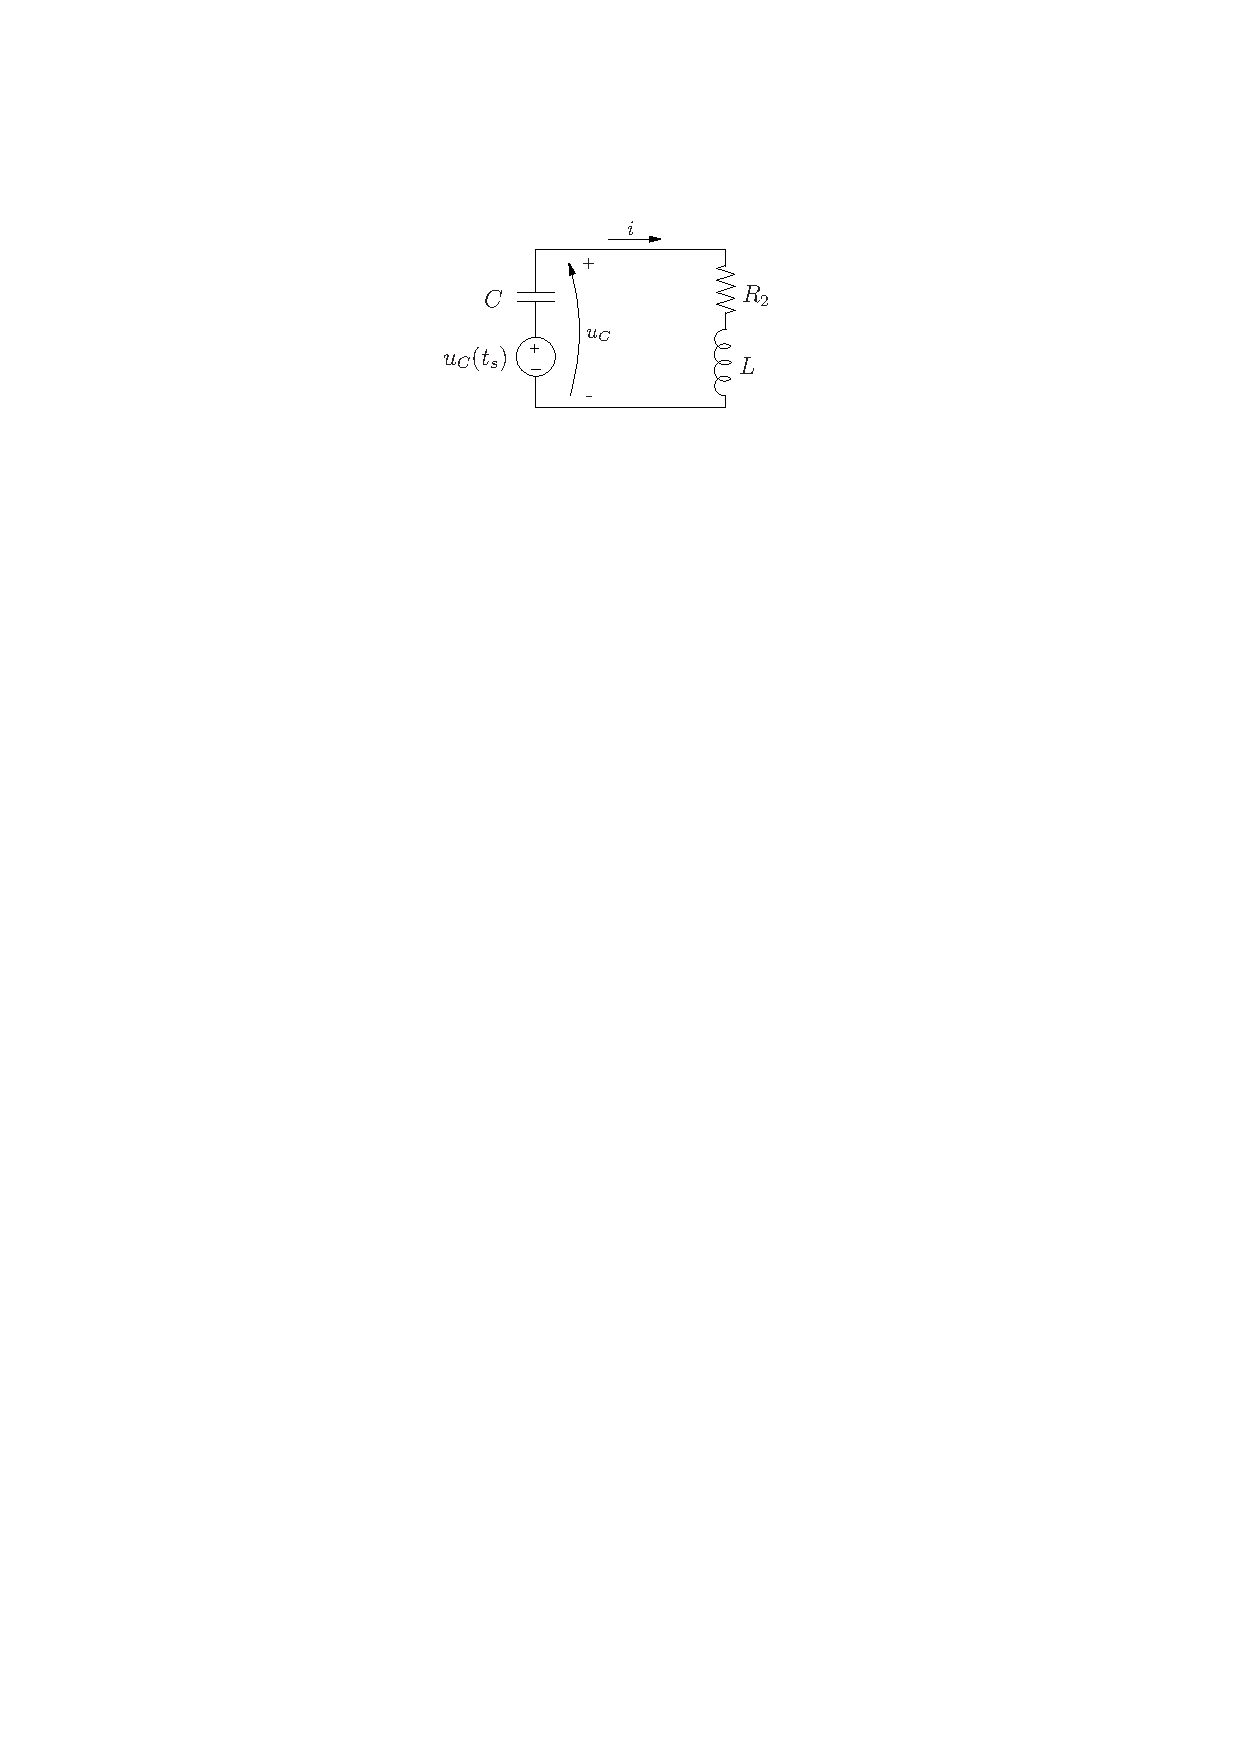
\includegraphics[width=\linewidth]{sol_exercices/ex3-8}
\end{center}
Le condensateur initialement chargé est remplacé
par son schéma équivalent constitué du condensateur $C$ initialement
relaxé connecté en série avec la source de tension $u_C(t_s)$, tension
initiale du condensateur.


Le circuit est un circuit RLC série dont on recherche la réponse
libre. Les paramètres $\alpha$, amortissement, et $\omega_0$, fréquence de
résonance sont donnés par :
\[\alpha=\frac{R_2}{2L}=1.25\ 10^5\quad , \quad
\omega_0=\frac{1}{\sqrt{LC}}=1.5811\, 10^5\]
On calcule :
\[\alpha^2-\omega_0^2=-9.375\, 10^9 <0\]
Le régime est de type oscillatoire amorti; les fréquences naturelles
du circuit sont :
\[s_{1,2}=-\alpha \pm j\sqrt{\omega_0^2-\alpha^2}=-\alpha \pm j\omega_d=
-1.25\, 10^5 \pm
j9.68\, 10^4\]

Le courant circulant dans le circuit s'écrit :
\begin{eqnarray*}
	i(t^{'})&=&\frac{u_C(t_s)}{\omega_d L}e^{-\alpha t^{'}}\sin (\omega_d
	t^{'})\\
	& = & 0.4648 e^{-1.25\, 10^5 t^{'}}\sin (9.68\, 10^4 t^{'})
\end{eqnarray*}
La tension aux bornes du condensateur se déduit comme suit :
\begin{eqnarray*}
	u_C(t^{'})& = &R_2 i(t^{'})+L\frac{di}{dt}\\
	& = & 116.19 e^{-1.25\, 10^5 t^{'}}\sin (9.68\, 10^4 t^{'}) + 90 e^{-1.25\, 10^5 t^{'}}\cos (9.68\, 10^4 t^{'})
\end{eqnarray*}
Cette expression peut aisément se mettre sous la forme générale :
\[ A\sin (\omega_d t + \phi)\]
En effet :
\begin{align*}
A\sin (\omega_d t + \phi)=A \cos \phi \sin \omega_d t + A\sin \phi \cos
\omega_d t
\end{align*}
On identifie :
\begin{align*}
A\sin \phi = 90 \quad , \quad A \cos \phi =  116.19\\
\mbox{et} \quad A = \sqrt{90^2+116.19^2}=147 \quad , \quad \phi =
\arctan \frac{90}{116.19}=0.66 \, \, \text{rad}
\end{align*}
Finalement :
\[u_C(t^{'})=147 e^{-1.25\, 10^5 t^{'}}\sin (9.68\, 10^4 t^{'}+0.66)\]
Remplaçant $t^{'}$ par $t-t_s$:
\[u_C(t)=147 e^{-1.25\, 10^5 (t-4.6\, 10^{-3})}\sin (9.68\, 10^4(t-4.6\, 10^{-3})+0.66)\]

\paragraph{Exercice~\ref{ex:2-9}}~\\%
Il faut distinguer les deux périodes~temporelles suivantes. 
\begin{enumerate}
	\item Période de lancement du moteur \: $0\leq t \leq t_d$.
	
	Durant cette période, la résistance de démarrage \ $R_d$ \ est
	insérée dans le circuit, l'interrupteur \ $\ell$ \ est ouvert.  On
	observe l'évolution du courant jusqu'à ce que celui-ci tombe sous
	15$\,$A. Soit \ $t_a$ \ cet instant. On attend 0.05$\,$s avant de
	mettre la résistance \ $R_d$ \ hors circuit et de fermer
	l'interrupteur \ $\ell$~. On a
	\[ t_d \, = \, t_a + 0.05~. \]           
	\item Résistance de démarrage hors service : \ $t>t_d$.
\end{enumerate}
\vspace*{1ex}

{\bf 1ère période~: \ $0\leq t < t_d$} 

Durant cette période, le circuit est celui représenté ci-dessous, avec :
\begin{eqnarray*}
	e(t) &=&E = 115 \\
	e_1(t) &=& 100(1-e^{-\frac{2}{3}t}) 
\end{eqnarray*}
\begin{center}
	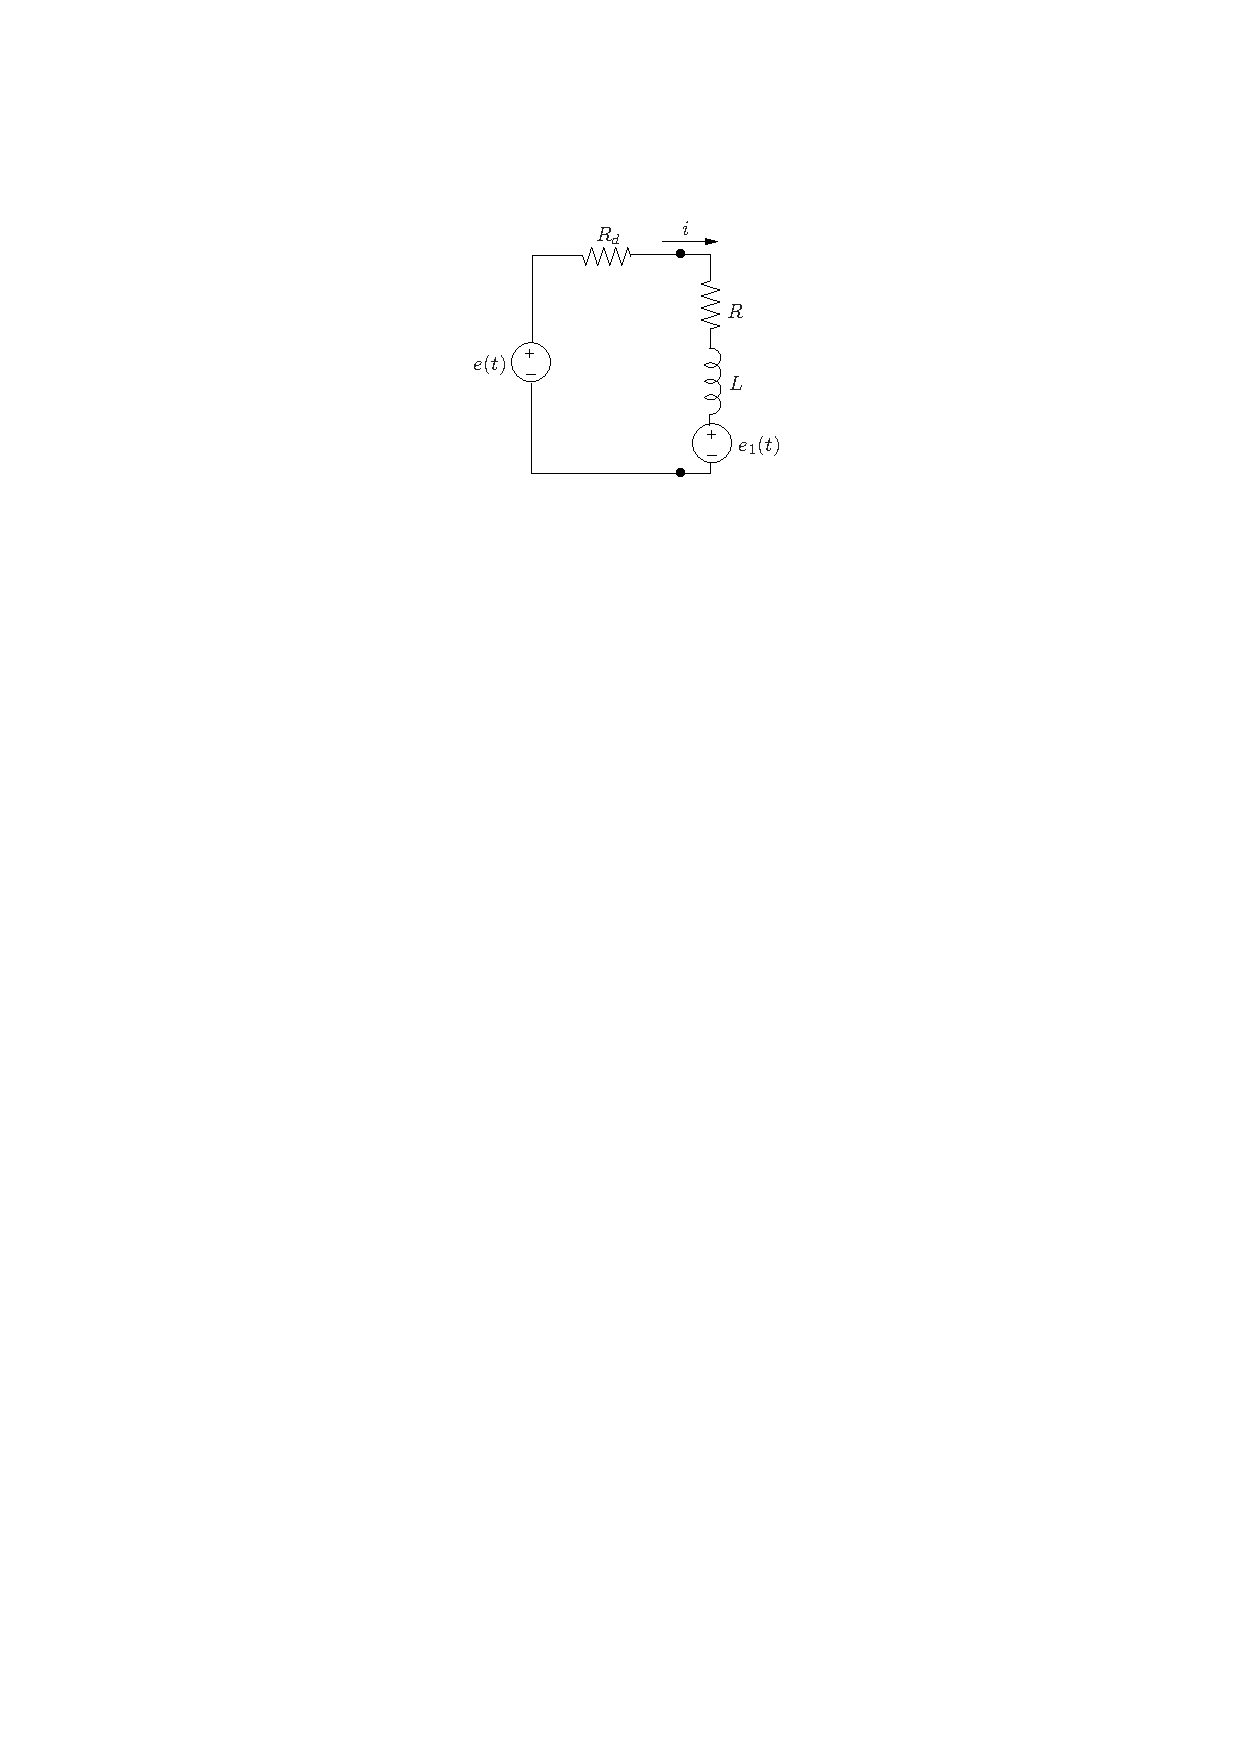
\includegraphics[width=\linewidth]{sol_exercices/ex3-9-1}
\end{center}

L'équation différentielle relative au courant $i(t)$ circulant dans le circuit s'écrit :

\[\frac{di}{dt}+\frac{R_{eq}}{L}i=\frac{e(t)-e_1(t)}{L}\]
avec $R_{eq}=R+R_d$

La solution générale de cette équation comprend d'une part la solution générale de l'équation homogène
\[i_h=Ae^{-\frac{t}{\tau_1}}\quad \text{avec la constante de temps} \quad \tau_1=\frac{L}{R_{eq}}=0.25\]
et d'autre part la solution particulière de l'équation non homogène qui peut s'écrire
\[i_p=B+Ce^{-\frac{2}{3}t} \, .\]
On identifie :
\begin{align*}
\frac{115-100+100e^{-\frac{2}{3}t}}{L}=\frac{R_{eq}}{L}(B+Ce^{-\frac{2}{3}t})-\frac{2}{3L}Ce^{-\frac{2}{3}t}\\
B=\frac{15}{R_{eq}}=3.75  \quad , \quad C=\frac{100}{R_{eq}-\frac{2}{3}}=30
\end{align*}
Finalement :
\[i(t)=i_h+i_p=Ae^{-\frac{t}{\tau_1}}+3.75 +30e^{-\frac{2}{3}t}.\]
La continuité du courant dans l'inductance en $t=0$ impose
\[i_L(0)=i(0)=A+3.75 +30=0 \quad \Rightarrow A=-33.75.\]


On déduit~:
\[ i(t) \: = \: 3.75 - 33.75 \, e^{-4t} + 30 \, e^{-\frac{2}{3} t} \,\,
, \quad 0\leq t < t_d~.\]

Cherchons maintenant l'instant $t_a$ tel que $i(t_a) =
15\,$A~. L'allure du courant $i(t)$ est représentée par
\begin{center}
	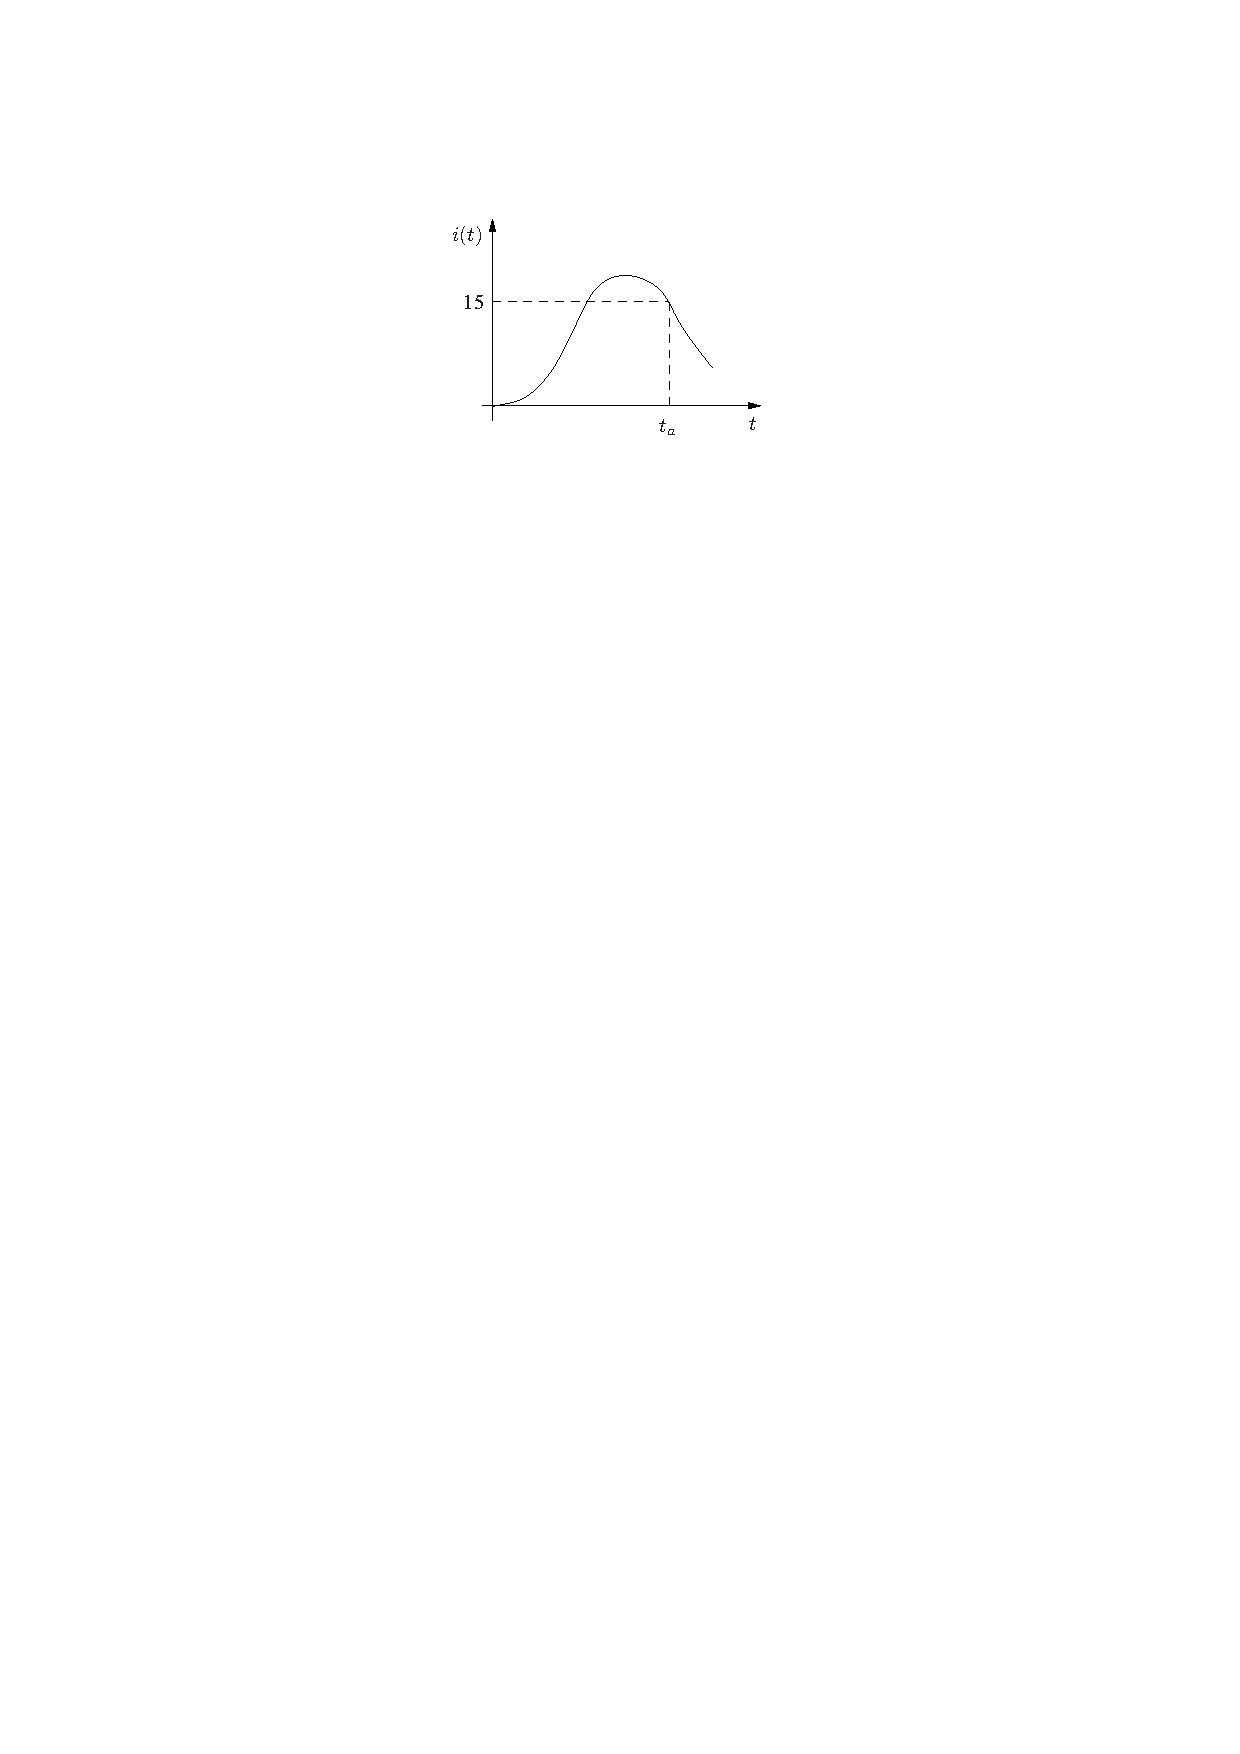
\includegraphics[width=\linewidth]{sol_exercices/ex3-9-2}
\end{center}
Il faut résoudre l'équation non linéaire~:
\[ 3.75 - 33.75 \, e^{-4t} + 30 \, e^{-\frac{2}{3}t} - 15 \: = \: 0 \: \equiv \ f(t) \: = \: 0~. \]
On a~:
\begin{eqnarray*}
	i(0) &=&0\\
	i(1) &=& 18.53\\
	i(2) &=& 11.65
\end{eqnarray*}
La solutions cherchée se trouve entre 1 et 2.  On peut soit procéder
par recherche dichotomique en divisant à chaque pas l'intervalle
encadrant la solution par 2, soit appliquer la méthode de
Newton. Celle-ci consiste à calculer la suite de points
\[ t^{(k+1)} \: = \: t^{(k)} - \frac{f(t^{(k)})}{f'(t^{(k)})} \quad k = 0,1,2... \]
jusqu'à ce que \ $\left| f(t^{(k)})\right| < \epsilon$~, où \ $\epsilon$ \ est une tolérance.

Soit \ $t^{(0)} = 1$~, on a~:
\[ f'(t) \: = \: 135\, e^{-4t} - 20 \, e^{-\frac{2}{3}t}~.\]
On calcule~:
\begin{eqnarray*}
	t^{(1)} &=& t^{(0)} - \frac{f(t^{(0)})}{f'(t^{(0)})} \: = \: 1.453\\
	t^{(2)} &=& t^{(1)} - \frac{f(t^{(1)})}{f'(t^{(1)})} \: = \: 1.458
\end{eqnarray*}
On a \ $f(t^{(2)}) = 8\, 10^{-4}$~. On juge la précision suffisante et
$t_a = t^{(2)} = 1.458$ s. Dès lors :
\[t_d=1.458+0.05=1.508\,\, \mbox{s}\]
A cet instant, le courant parcourant le circuit vaut \ $i\, (1.508) =
14.647\,$A~.

\vspace{\baselineskip}
{\bf 2ème période~: \ $ t \geq  t_d$}

Fixons une nouvelle origine des temps en \ $t=t_d$~. Pour cela, on introduit le changement de variable
\[ t' \, = \, t - t_d~. \]
A l'instant de basculement $t_d$, l'inductance est parcourue par le courant \ $i(t_d)$~.
Durant cette période, le circuit prend la forme de 
\begin{center}
	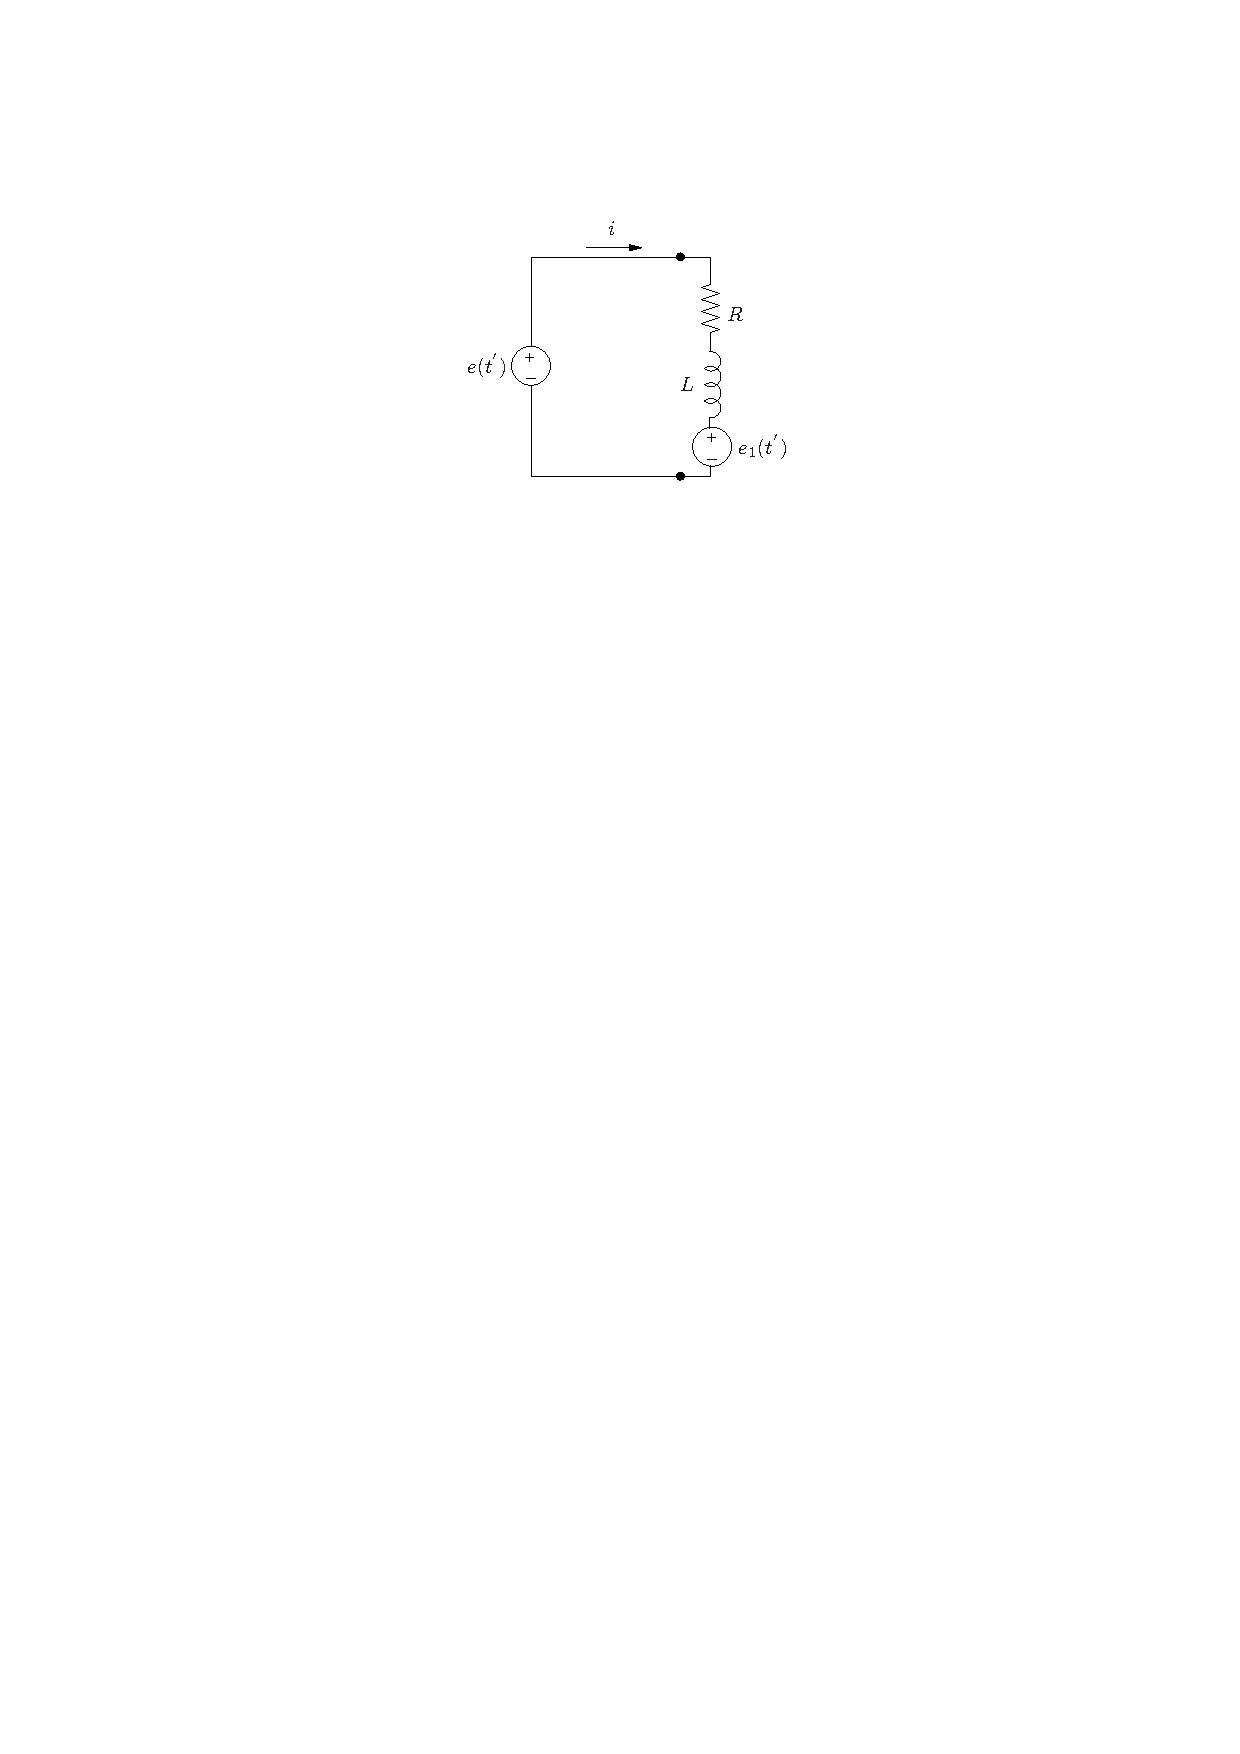
\includegraphics[width=\linewidth]{sol_exercices/ex3-9-3}
\end{center}


Les excitations \ $e$ et $e_1$ \ s'écrivent pour la période \ $t> t_d$~:
\begin{eqnarray*}
	e(t') &=& E=115 \\
	e_1(t') &=&100 \left( 1-e^{-\frac{2}{3}(t'+t_{d})} \right)\\
\end{eqnarray*}
L'équation différentielle relative au courant $i(t^{'})$ circulant dans le circuit s'écrit :
\[\frac{di}{dt}+\frac{R}{L}i=\frac{e(t^{'})-e_1(t^{'})}{L}\]

On calcule pour cette période temporelle~:
\begin{eqnarray*} 
	i(t^{'}) &=&  Ae^{-\frac{t^{'}}{\tau_2}}+B+Ce^{-\frac{2}{3}t^{'}}
\end{eqnarray*}
avec la constante de temps $\tau_2=\frac{L}{R}=0.5$.
On identifie :
\begin{align*}
\frac{115-100}{L}=\frac{R}{L}B\quad \Rightarrow \quad B=7.5\\
\frac{100e^{-\frac{2}{3}t_d}}{L}=\frac{R}{L}B -\frac{2}{3}C \quad \Rightarrow \quad C=27.44\\
i(t^{'}=0)=i_L(t_d)=14.647 \quad \Rightarrow \quad A=-20.3
\end{align*}


Le courant, exprimé selon la nouvelle variable temporelle $t^{'}$, s'écrit~:
\[ i(t') \: = \: 7.5 - 20.3 \, e^{-2t'} + 27.44 \,
e^{-\frac{2}{3}t'} \,\, , \quad t'>0 \]
où, en fonction de \ $t$, en rempla{c}ant \ $t'$ \ par \ $t-t_d$~:
\begin{eqnarray*}
	i(t) &=& 7.5 - 20.297 \, e^{-2(t-t_d)} + 27.44 \,
	e^{-\frac{2}{3}(t-t_d)} \,\, , \quad t > t_d\\
	&=& 7.5 - 414.2 \, e^{-2t} + 75 \, e^{-\frac{2}{3}t}  \,\, , \quad t > t_d.
\end{eqnarray*}

Si la résistance de démarrage n'était pas  insérée dans le circuit,
le courant, pour toute la période temporelle $t \geq  0$,
s'obtiendrait comme suit :
\begin{eqnarray*}
	i^{'}(t)=Ae^{-\frac{t}{\tau_2}}+B+Ce^{-\frac{2}{3}t}
\end{eqnarray*}
On identifie :
\[ B=7.5 \quad , \quad C=75 \quad , \quad A=-82.5\]
et
\[i^{'}(t)  =  7.5 - 82.5 e^{-2t} + 75 e^{-\frac{2}{3}
	t} \,\, , \quad t\geq 0\]

La figure ci-dessous compare les 2 courants $i(t)$ et $i^{'}(t)$ 
et montre l'influence de la résistance \ $R_d$ \ qui permet de limiter
l'amplitude du courant dans les premiers instants qui  suivent le démarrage
du moteur.
\begin{center}
	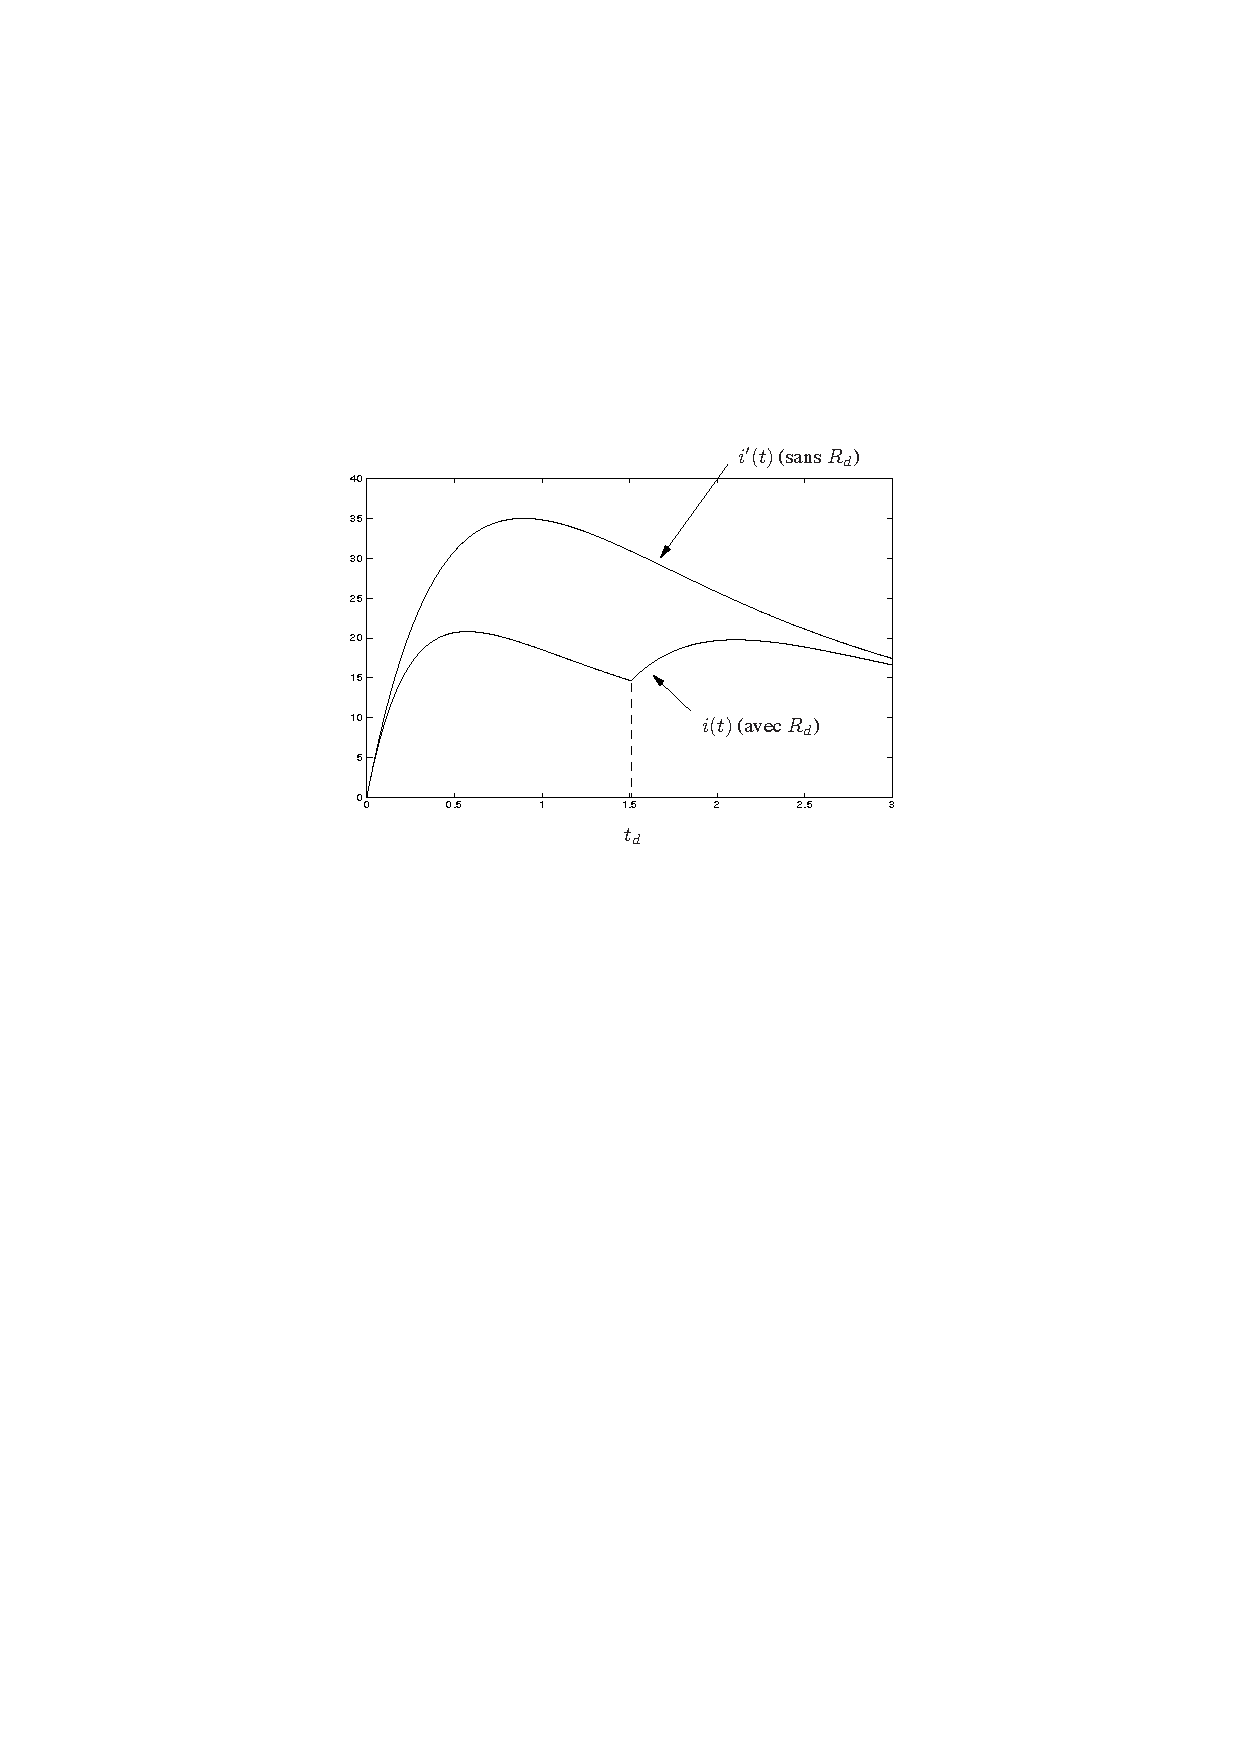
\includegraphics[width=\linewidth]{sol_exercices/ex3-9-4}
\end{center}


\paragraph{Exercice~\ref{ex:2-11}}~\\%
\begin{center}
	\begin{circuitikz}[european voltages]
		\draw
		(0,0)
		to[battery1, l=$E$] ++(0,3)
		to[R, l^=$R_1$, i>=$i_1$, -*] ++(4,0) coordinate (A)
		to[short] ++(3,0)
		to[C, l_=$C_1$, v^=$v_{C_1}$, i_=$i_3$] ++(0,-3)
		--(0,0)
		(A)
		to[R, l^=$R_2$,	 i=$i_2$, -*] ++(0,-3)
		;
	\end{circuitikz}
\end{center}
Conditions initiales :
\begin{itemize}
	\item  $v_{C_1}(0-) = v_0$
	\item $i_1(0-) = i_2(0-) = i_3(0-) = 0$
\end{itemize}

\begin{align}
i_1 &= i_2 + i_3 &\text{ PLK}\\
R_2 i_2 &= v_{C_1} &\text{ SLK}\\
R_1 i_1 &= E - v_{C_1} &\text{ SLK}\\
i_3 &= C_1 \frac{dv_{C_1}}{dt}
\end{align}
Donc 
\begin{align}
C_1 \frac{dv_{C_1}}{dt} &= \frac{E - v_{C_1}}{R_1} - \frac{v_{C_1}}{R_2} \\
C_1 \frac{dv_{C_1}}{dt} + v_{C_1} \left(\frac{1}{R_1}+\frac{1}{R_2}\right)&= \frac{E}{R_1} \\
\frac{dv_{C_1}}{dt} + \frac{1}{\tau_1} v_{C_1} &= \frac{E}{\tau_2}
\end{align} 
Avec
\begin{align}
\tau_1 &= \frac{C_1R_1R_2}{R_1+R_2}\\
\tau_2 &= C_1R_1
\end{align}
L'équation homogène 
$$\frac{dv_{C_1}}{dt} + \frac{1}{\tau_1} v_{C_1} = 0$$
a pour solution
$$v_{C_1}^h(t) = K_1 e^{s_1t}$$
avec $s_1 = \tau_1^{-1}$.
Une solution particulière de 
$$\frac{dv_{C_1}}{dt} + \frac{1}{\tau_1} v_{C_1} = \frac{E}{\tau_2}$$
est 
$$v_{C_1}^p(t) = K_2$$
avec $$K_2=\frac{\tau_1 E} {\tau_2} = \frac{R_2}{R_1+R_2} E.$$
Donc 
$$ v_{C_1}(t) = K_1 e^{-t/\tau_1} + \frac{R_2}{R_1+R_2} E$$ 
Tenant compte de $v_{C_1}(0-) = v_0$ et par continuité de la tension aux bornes du condensateur, on obtient $K_1 = v_0 - \frac{R_2}{R_1+R_2} E$.
Et donc finalement 
$$ v_{C_1}(t) = \left(v_0 - \frac{R_2}{R_1+R_2} E\right) e^{-t/\tau_1} + \frac{R_2}{R_1+R_2} E$$ 
En régime établi, c'est simplement la formule du diviseur de tension qui s'applique, car aucun courant ne passe plus par la branche du condensateur.

\vspace{2cm}

\textbf{Alternativement}, on aurait pu remplacer le condensateur initialement chargé par un condensateur relaxé en série avec une source (indépendante) de tension de valeur $v_0$.
\begin{center}
	\begin{circuitikz}[european voltages]
		\draw
		(0,0)
		to[battery1, l=$E$] ++(0,3)
		to[R, l^=$R_1$, i>=$i_1$, -*] ++(4,0) coordinate (A)
		to[short] ++(3,0)
		to[C, l_=$C_1$, v^=$v_{C_1}$, i_=$i_3$] ++(0,-2)
		to[battery1,l=$-v_0$] ++(0,-1)
		--(0,0)
		(A)
		to[R, l^=$R_2$,	 i=$i_2$, -*] ++(0,-3)
		;
	\end{circuitikz}
\end{center}
Conditions initiales :
\begin{itemize}
	\item  $v_{C_1}(0-) = \textcolor{red}{0}$
	\item $i_1(0-) = i_2(0-) = i_3(0-) = 0$
\end{itemize}

\begin{align}
i_1 &= i_2 + i_3 &\text{ PLK}\\
R_2 i_2 &= v_{C_1} \textcolor{red}{+ v_0} &\text{ SLK}\\
R_1 i_1 &= E - v_{C_1} \textcolor{red}{- v_0} &\text{ SLK}\\
i_3 &= C_1 \frac{dv_{C_1}}{dt}
\end{align}
Donc 
\begin{align}
C_1 \frac{dv_{C_1}}{dt} &= \frac{E - v_{C_1} \textcolor{red}{- v_0}}{R_1} - \frac{v_{C_1}\textcolor{red}{+v_0}}{R_2} \\
C_1 \frac{dv_{C_1}}{dt} + v_{C_1} \left(\frac{1}{R_1}+\frac{1}{R_2}\right)&= \frac{E}{R_1} - \textcolor{red}{\frac{v_0}{R_1} - \frac{v_0}{R_2}}\\
\frac{dv_{C_1}}{dt} + \frac{1}{\tau_1} v_{C_1} &= \frac{E}{\tau_2} \textcolor{red}{- \frac{v_0}{\tau_1}}
\end{align} 
Avec
\begin{align}
\tau_1 &= \frac{C_1R_1R_2}{R_1+R_2}\\
\tau_2 &= C_1R_1
\end{align}
L'équation homogène 
$$\frac{dv_{C_1}}{dt} + \frac{1}{\tau_1} v_{C_1} = 0$$
a pour solution
$$v_{C_1}^h(t) = K_1 e^{s_1t}$$
avec $s_1 = \tau_1^{-1}$.
Une solution particulière de 
$$\frac{dv_{C_1}}{dt} + \frac{1}{\tau_1} v_{C_1} = \frac{E}{\tau_2} \textcolor{red}{- \frac{v_0}{\tau_1}}$$
est 
$$v_{C_1}^p(t) = K_2$$
avec $$K_2 = \frac{R_2}{R_1+R_2} E  \textcolor{red}{- v_0}.$$
Donc 
$$ v_{C_1}(t) = K_1 e^{-t/\tau_1} + \frac{R_2}{R_1+R_2} E \textcolor{red}{- v_0}.$$ 
Tenant compte de $v_{C_1}(0-) = 0$ et par continuité de la tension aux bornes du condensateur, on obtient $$K_1 = v_0 - \frac{R_2}{R_1+R_2} E.$$
Finalement 
$$ v_{C_1}(t) = \left(v_0 - \frac{R_2}{R_1+R_2} E\right) e^{-t/\tau_1} + \frac{R_2}{R_1+R_2} E \textcolor{red}{- v_0}$$
Le terme additionnel $- v_0$ compense la source de tension introduite.

\paragraph{Exercice~\ref{ex:2-14}}~\\%

\begin{enumerate}
	\item Le point 1 nous dit que nous sommes en régime établi, la bobine se comporte comme un court-circuit et ne présente aucune ddp. Le courant $i$ est dicté par 
	$$i(t) = \frac{120-100}{2} = 10 \ A, \ t < 0.$$
	\item Ensuite, nous avons 
	$$e_1(t) - R i(t) - L \frac{di(t)}{dt} - 100 = 0,$$
	avec $i(0^-) = 10 A$.
	Donc 
	$$\frac{di(t)}{dt} + \frac{R}{L} i(t)  = \frac{1}{L} (100 - e_1(t)).$$
	Cette équation admet comme solution particulière $i_p(t) = K_1 + K_2 e^{-10t}$.
	Identifions les paramètres :
	\begin{align*}
	\frac{1}{L} (100 - e_1(t)) &= -10 K_2 e^{-10t} + \frac{R2}{L} (K_1 + K_2 e^{-10t}) \\
	&= K_2 e^{-10t} (\frac{R2}{L} -10 ) + \frac{R2}{L} K_1.
	\end{align*}
	En identifiant la partie constante et la partie en $e^{-10t}$, on obtient 
	$$i_p(t) = -50-40 e^{-10t}.$$
	
	Une solution de l'équation homogène est $$i_h(t) = K_3 e^{-\frac{t}{\tau}},$$  avec $\tau = 0.25 s$. Comme par continuité $i(0^+) = 10 A$, on a
	$$K_3 e^{-4t} -50-40 e^{-10t} = 10$$
	en $t = 0^+$, donc $K_3 = 100$.
	\item 
	Le courant s'annule à $t_0$ tel que $$100 e^{-4t} -50-40 e^{-10t_0} = 0,$$
	ce qui donne $t_0 \approx 0.12 s$. 
	\item En $t_1 \approx 0.17s$, le courant vaut $-6.65 A$. C'est la condition initiale de cette dernière phase. Si on translate l'origine du temps en $t_1$, on a maintenant une solution de type réponse libre
	$$\frac{di(t)}{dt} + \frac{R}{L} i(t)  = \frac{20}{L},$$
	et donc $i(t) = \frac{20}{R} + K e^{-\frac{t}{\tau}}$ avec $\tau = \frac{L}{R}$, et donc $$K = -6.65 - \frac{20}{R} = -16.65.$$
	Finalement, et en re-translatant l'origine des temps,  $i(t) = 10 - 16.65 e^{-4(t-t_1)}$.
\end{enumerate}
La dynamique est illustrée à la figure ci-dessous.
\begin{center}
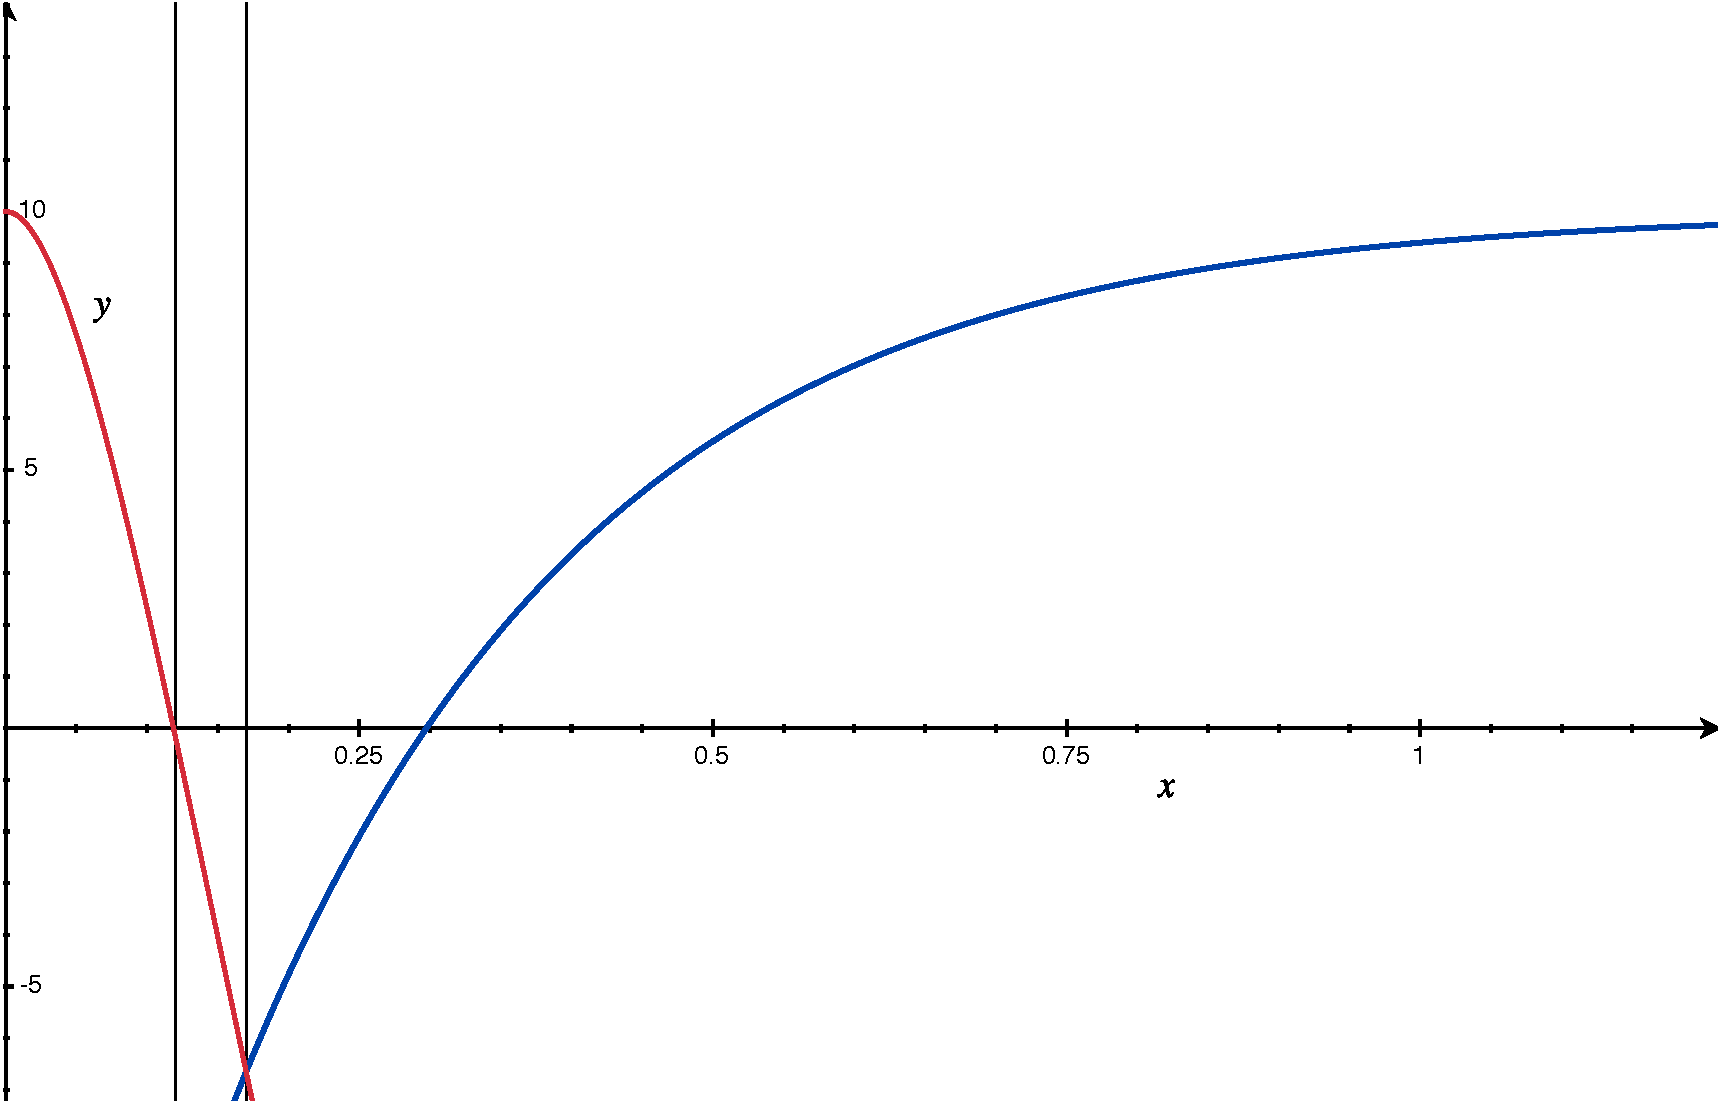
\includegraphics[width=0.7\linewidth]{figs/ex_RLC}
\end{center}
